\documentclass[12pt,a4paper]{amsart}
\renewcommand{\baselinestretch}{1.8} 
\usepackage[utf8]{inputenc}
\usepackage[english,russian]{babel}
\usepackage{amsfonts, amsmath, amssymb, amsthm, amscd, hyperref, mathrsfs, mathtext}
\usepackage{a4wide}
\usepackage{tikz}
\usepackage{graphicx, epsfig}
\usepackage{subcaption}
\usepackage{setspace}
\usepackage{cleveref}
\usepackage{hyperref}
\usepackage{tabulary}

\usepackage[left=3cm,right=2cm, top=2cm, bottom=2cm,bindingoffset=0cm]{geometry}

\usepackage{anysize}

\renewcommand{\thesubfigure}{(\alph{subfigure})}
\captionsetup[sub]{labelformat=simple}

\newenvironment{comment}{}{}

\usepackage{hyperref}
\hypersetup{
	colorlinks   = true, %Colours links instead of ugly boxes
	urlcolor     = blue, %Colour for external hyperlinks
	linkcolor    = blue, %Colour of internal links
	citecolor   = red %Colour of citations
}

\usepackage{anysize}


\newenvironment{nouppercase}{%
	\let\uppercase\relax%
	\renewcommand{\uppercasenonmath}[1]{}}{}

\relpenalty=100
\binoppenalty=1000

\setlength{\textwidth}{\paperwidth}
\addtolength{\textwidth}{-40mm}
\calclayout

\begin{document}


{\setstretch{1.0}
\begin{titlepage}

\begin{center}
	Министерство образования и науки Российской Федерации
	\vspace{0.4cm}
	
	Федеральное государственное автономное образовательное учреждение высшего профессионального образования
	\vspace{0.4cm}
	
	<<Московский физико-технический институт (государственный университет)>>
	\vspace{0.4cm}
	
	Факультет инноваций и высоких технологий
	\vspace{0.4cm}
	
	Кафедра анализа данных
	\vspace{0.7cm}
	
\end{center}

\vspace{1.4cm}

\begin{center}
	\Large Персиянов Дмитрий Андреевич
\end{center}

\vspace{0.8cm}

\begin{center}
	\Huge Обучение с подкреплением нейросетевых диалоговых моделей \linebreak для вспомогательных целей
\end{center}

\vspace{1.3cm}

\begin{center}
	\bf Выпускная квалификационная работа бакалавра
\end{center}

\vspace{1.8cm}

\begin{center}
	Направление подготовки: 01.03.02 Прикладные математика и информатика
\end{center}

\vspace{0.8cm}

\vspace{2.0cm}

Зам. зав. кафедрой \verb"              " \underline{\quad \quad \quad \quad \quad \quad \quad}
\verb"        "
%/Райгородский А.М./
/Бунина Е.И./

Научный руководитель \verb"           " \underline{\quad \quad \quad \quad \quad \quad \quad}
\verb"        "
/Устюжанин А.Е./

Студент \verb"                        " \underline{\quad \quad \quad \quad \quad \quad \quad}
\verb"        "
/Персиянов Д.А./

\vspace{1.0cm}

\hbox to \textwidth
{
	\hss г. Москва \hss
}
\hbox to \textwidth
{
	\hss 2017 \hss
}

\end{titlepage}




\title{Обучение с подкреплением нейросетевых диалоговых моделей \linebreak для вспомогательных целей}

\author{Д.А.~Персиянов}

\email{persiyanov@phystech.edu}
\address{Персиянов Дмитрий, каф. анализа данных, Московский физико-технический институт (государственный университет)}


\begin{abstract}
В современном мире большую популярность набрали диалоговые модели на основе рекуррентных нейронных сетей. Обучение моделей происходит на огромных корпусах текстов. Однако, для применения их в прикладных задачах (чат-поддержка в банке, персональный помощник пользователя и т.д.) необходимо, чтобы модель соответствовала определенным, иногда жестким требованиям. В работе предлагается способ дообучения диалоговых моделей под эти требования на основе policy-gradient алгоритмов обучения с подкреплением. Предложенный подход не требует большого количества данных и не накладывает ограничений на их вид, в отличие от дообучения по методу максимального правдоподобия. На примере двух задач: запрета обсценной лексики в ответе и требования отвечать в ''стиле'' какой-либо персоны демонстрируется эффективность метода.
\end{abstract}


\begin{nouppercase}
\maketitle
\end{nouppercase}

\begin{large}
	\tableofcontents
\end{large}

}

\pagebreak
\section{Введение}

Люди все больше взаимодействуют с компьютером через естественные диалоговые интерфейсы, которые помогают пользователю с различными повседневными задачами. Такие системы называют целеориентированными (англ. goal-oriented) диалоговыми системами. Классические подходы для построения целеориентированных диалоговых систем (Amazon Alexa, Microsoft Cortana, Google Assistant, Apple Siri, Яндекс Алиса) основаны на модуле отслеживании состояния диалога (англ. dialog state tracking), а также модуле распознавания естественного языка (англ. natural language understanding). Обучение этих компонент требует данных из предметной области со сложной разметкой (\cite{DBLP:journals/corr/ZhaoE16} \cite{DBLP:journals/corr/MrksicSTGSVWY15} \cite{DBLP:journals/corr/Perez16}).

С другой стороны, бурное развитие получили диалоговые нейросетевые модели, направленные на общение на общие темы (англ. open-domain). Их можно разделить на две категории: к первой относятся генеративные модели, основанные на рекуррентных сетях (\cite{DBLP:journals/corr/VinyalsL15} \cite{DBLP:journals/corr/LiGBGD16} \cite{DBLP:journals/corr/SerbanSBCP15}), ко второй модели, ранжирующие большой индекс возможных ответов (\cite{semantic-parsing-for-single-relation-question-answering} \cite{learning-deep-structured-semantic-models-for-web-search-using-clickthrough-data}). Обучение происходит на огромных датасетах с диалогами и структурированная разметка, как правило, не требуется. В данной работе рассматриваются только генеративные диалоговые модели, для краткости будем называть их просто диалоговыми моделями (системами).

Для обучения диалоговых моделей требуются выборки с миллионами пар контекст-ответ, над которыми часто нет контроля. Таким образом модель может обучиться отвечать не так, как хотелось бы. Например, в ответах может присутствовать обсценная лексика или модель может отвечать оскорбительно на контексты, касающиеся культурных, расовых проблем и т.п. В связи с этим возникает задача обучения модели так, чтобы она удовлетворяла такого рода требованиям.

Следующая задача, возникающая при отсутствии большого специфичного датасета с репликами, состоит в том, чтобы научить модель общаться как какая-то персона и отвечать в стиле этой персоны. Обе вышеперечисленные задачи можно сформулировать на языке обучения с подкреплением, то есть в виде функции наград за сгенерированный ответ.

Интерес к обучению с подкреплением снова вырос в последние несколько лет. Успех его интеграции с глубоким обучением подкрепляется статьями группы DeepMind  (\cite{DBLP:journals/corr/MnihKSGAWR13} \cite{silver2016mastering}). Обучение с подкреплением позволяет работать с недифференцируемыми функциями наград, что открывает широкие возможности применения таких алгоритмов для дообучения диалоговых моделей (\cite{DBLP:journals/corr/AsadiW16} \cite{DBLP:journals/corr/BordesW16} \cite{DBLP:journals/corr/LiMRGGJ16} \cite{DBLP:journals/corr/LiptonGLLAD16} \cite{DBLP:journals/corr/PengLLGCLW17}).

В данной работе предлагается подход, основанный на глубоком обучении с подкреплением и требующий небольшое количество времени и данных для обучения моделей. Рассматриваются задачи запрета списка слов для модели, а также задача генерации ответов в стиле какой-либо персоны. Предложенный подход значительно превосходит бейзлайны без обучения с подкреплением.

\pagebreak
\section{Нейросетевые диалоговые модели}

В данной главе представлены базовые знания о рекуррентных сетях и sequence-to-sequence подходе для построения диалоговых систем.

\subsection{Рекуррентные нейронные сети}

Рекуррентные нейронные сети органично подходят для работы с данными, в которых наблюдается последовательная структура. Примерами таких данных являются тексты (последовательность слов), временные ряды, видеоряды (последовательность кадров), звук.

\begin{figure}[h]
	\caption{Схематичное устройство рекуррентной нейронной сети.}
	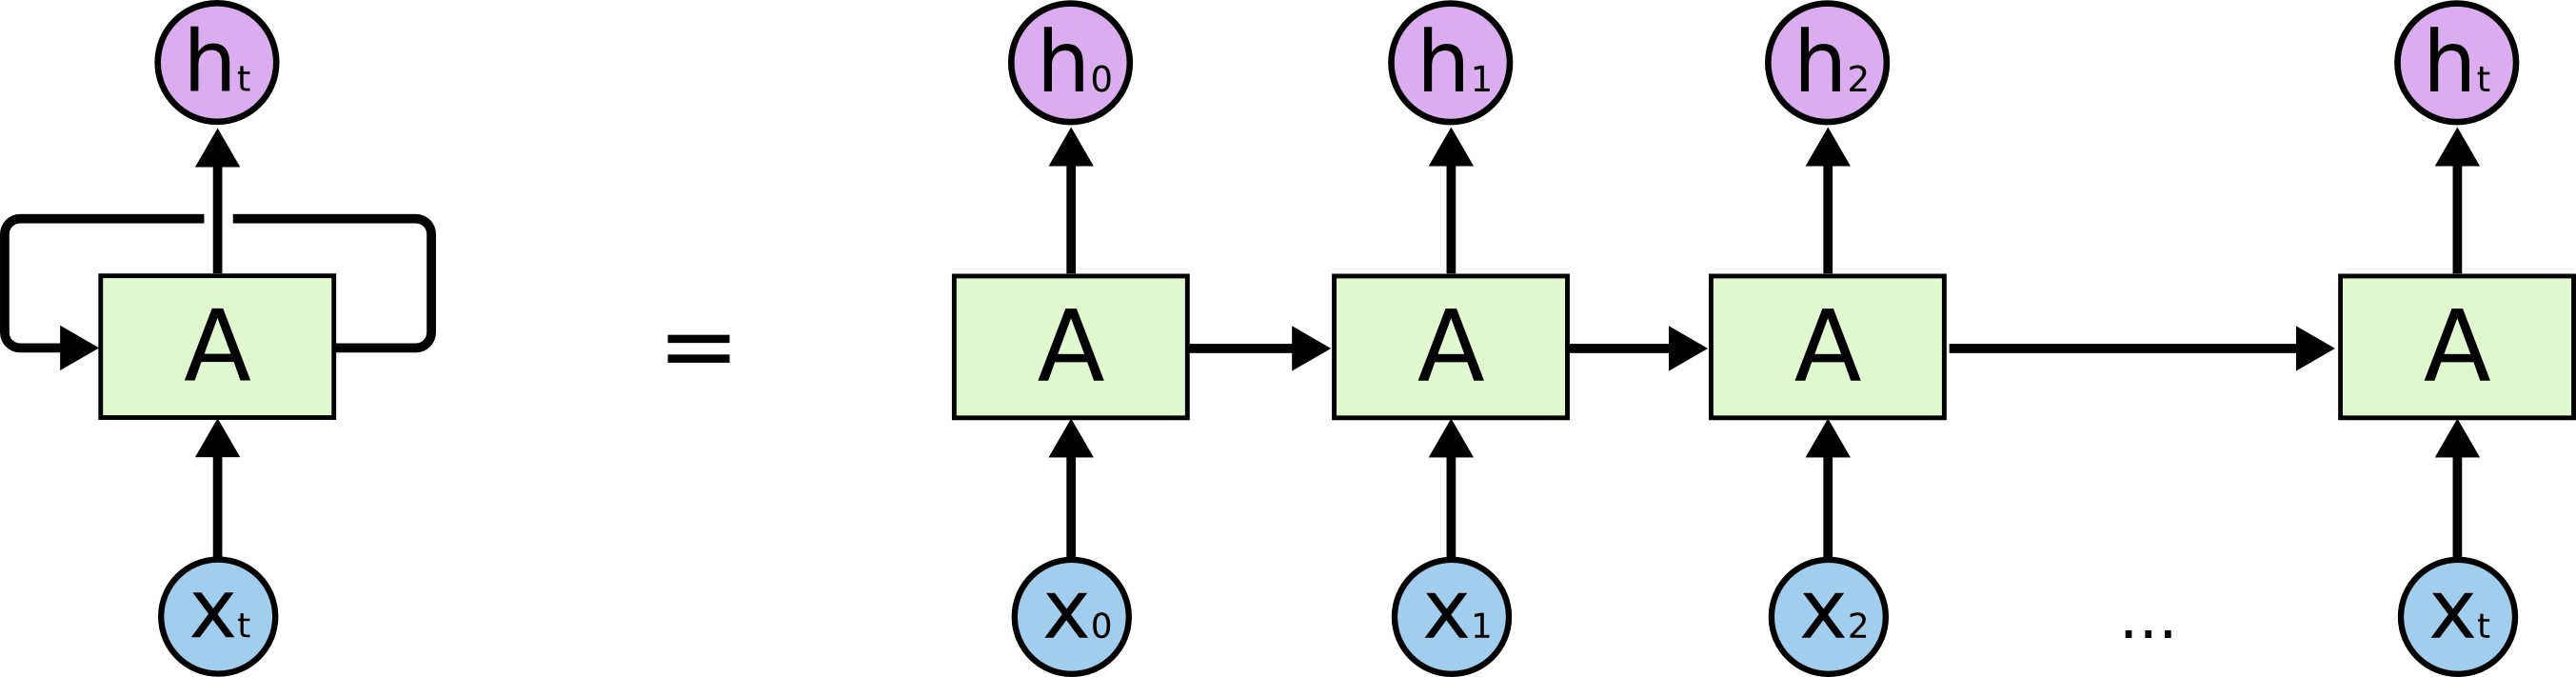
\includegraphics[width=\textwidth]{imgs/RNN-unrolled.png}
	\label{fig:rnn-overview}
	\centering
\end{figure}

На Рис. \ref{fig:rnn-overview} обозначено примерное устройство рекуррентной сети. Более формально, на вход сети подается последовательность входных векторов $\mathbf{x} = \lbrace \mathbf{x_1}, \mathbf{x_2}, \dots, \mathbf{x_n}\rbrace$, а она в свою очередь обрабатывает эту последовательность, поддерживая вектор скрытого состояния $\mathbf{h_t}$. Изначально (до обработки первого вектора входной последовательности) скрытое состояние инициализируется, например, нулями ($\mathbf{h_0} = \mathbf{0}$). Скрытое состояние обновляется следующим образом:

\begin{equation} \label{eq:vanilla-rnn-h}
\mathbf{h_t} = \sigma (W^{(hh)}\mathbf{h_{t-1}}+W^{(hx)}\mathbf{x_t}),
\end{equation}

где $\sigma(x) = \frac{1}{1+\exp^{-x}}$ -- сигмоидная функция активации (для вектора применяется поточечно), а $W^{(hh)},~W^{(hx)}$ -- матрицы обучаемых параметров рекуррентного слоя. Из формулы \eqref{eq:vanilla-rnn-h} понятно, что размерность вектора скрытого состояния можно варьировать и тем самым влиять на архитектуру сети и количество обучаемых параметров. В экспериментах в данной работе эта размерность будет равна 1024.

Преимущество рекуррентной архитектуры в возможности предсказывать целевые переменные различных типов. В общем случае, если входной последовательности $\mathbf{x} = \lbrace \mathbf{x_1}, \mathbf{x_2}, \dots, \mathbf{x_n}\rbrace$ соответствует последовательность $y = \lbrace y_1, y_2, \dots, y_n\rbrace$ целевых переменных для каждого элемента $\mathbf{x_t}$, как, например, в задаче POS-таггинга, предсказать такую последовательность $\hat{y} = \lbrace \hat{y}_1, \hat{y}_2, \dots, \hat{y}_n\rbrace$ можно, используя скрытое состояние на каждом шаге:

\begin{equation} \label{eq:vanilla-rnn-yhat}
\hat{y}_t = \text{softmax}(U\mathbf{h_t}),
\end{equation}

где $\text{softmax}(\mathbf{v}) = \big(\frac{e^{v_1}}{\sum e^{v_i}}, \frac{e^{v_2}}{\sum e^{v_i}}, \dots, \frac{e^{v_n}}{\sum e^{v_i}}\big)$ -- классификационная функция активации, $U \in \mathbb{R}^K \times \mathbb{R}^{dim\mathbf{h_t}}$ -- матрица параметров, $K$ -- количество классов.

Также возможно предсказывать целевую переменную после обработки входной последовательности, используя финальное скрытое состояние сети $\mathbf{h_n}$.

\begin{figure}[!h]
	\begin{subfigure}{0.31\textwidth}
		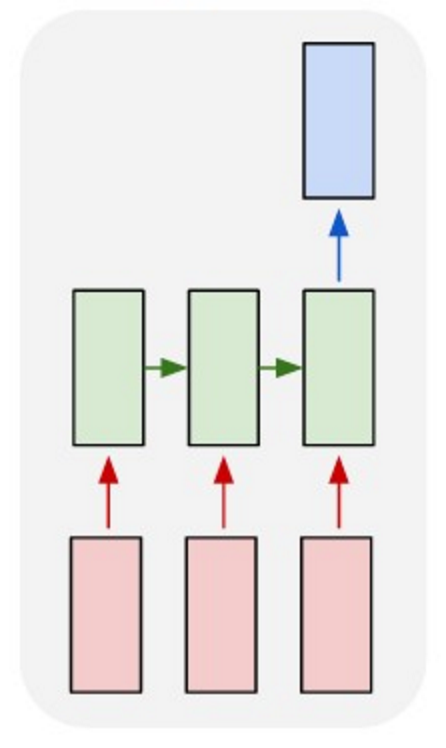
\includegraphics[scale=0.5]{imgs/rnn-many-to-one.png}
		\caption{}
		\label{fig:rnn-variants-many-to-one}
	\end{subfigure}\hfill
	\begin{subfigure}{0.31\textwidth}
		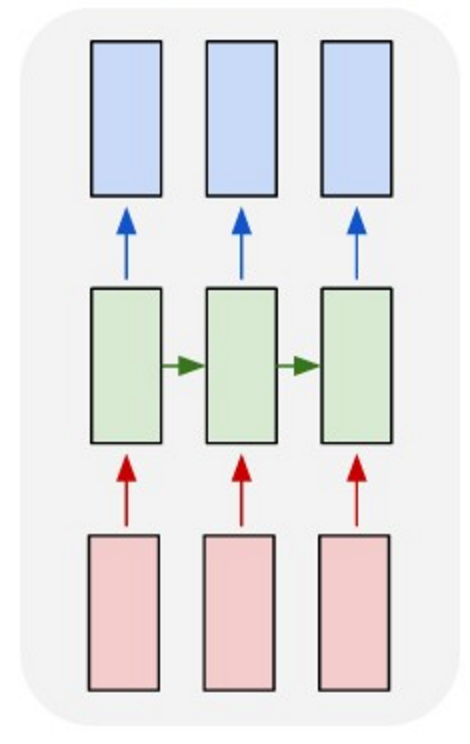
\includegraphics[scale=0.5]{imgs/rnn-many-to-many-2.png}
		\caption{}
		\label{fig:rnn-variants-many-to-many}
	\end{subfigure}\hfill
	\begin{subfigure}{0.31\textwidth}
		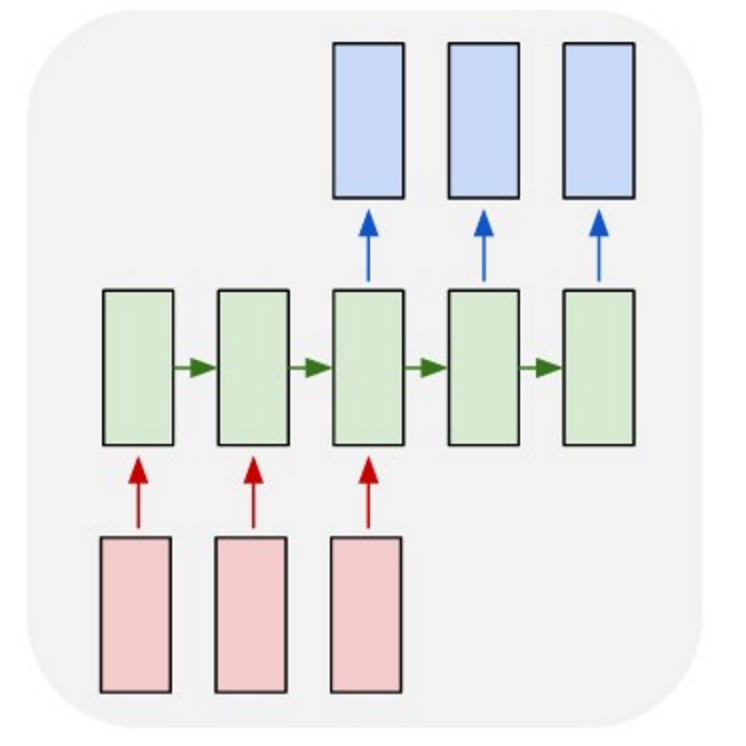
\includegraphics[scale=0.47]{imgs/rnn-many-to-many.png}
		\caption{}
		\label{fig:rnn-variants-many-to-many-seq2seq}
	\end{subfigure}
	\caption{Варианты структуры целевой переменной и ее предсказание.}
	\label{fig:rnn-variants}
\end{figure}

Таким образом, рекуррентные сети подходят для широкого спектра задач предсказания на данных, имеющих последовательную структуру. На Рис. \ref{fig:rnn-variants-many-to-one} проиллюстрирован вариант предсказания целевой переменной после обработки входной последовательности, на Рис. \ref{fig:rnn-variants-many-to-many} предсказание последовательности целевых переменных на каждом шаге, на Рис. \ref{fig:rnn-variants-many-to-many-seq2seq} предсказание последовательности целевых переменных после обработки входной последовательности.

Вышеупомянутый способ \eqref{eq:vanilla-rnn-h} (т.н. ''vanilla'' ячейка) обновления скрытого состояния сети имеет свои недостатки, в числе которых популярная проблема затухания и ''взрыва'' градиентов (\cite{Hochreiter:1997:LSM:1246443.1246450}). В связи с этим стали популярны другие виды рекуррентных ячеек, такие как LSTM и GRU. В данной работе во всех экспериментах используются ячейки LSTM, обновление в которых происходит следующим образом:

\begin{align*} \label{eq:lstm-equations}
\mathbf{i_t} &= \sigma(W^{(i)}\mathbf{x_t} + U^{(i)}\mathbf{h_{t-1}}) \\
\mathbf{f_t} &= \sigma(W^{(f)}\mathbf{x_t} + U^{(f)}\mathbf{h_{t-1}}) \\
\mathbf{o_t} &= \sigma(W^{(o)}\mathbf{x_t} + U^{(o)}\mathbf{h_{t-1}}) \\
\mathbf{\tilde{c_t}} &= \text{tanh}(W^{(c)}\mathbf{x_t} + U^{(c)}\mathbf{h_{t-1}}) \\
\mathbf{c_t} &= \mathbf{f_t} \circ \mathbf{c_{t-1}} + \mathbf{i_t} \circ \mathbf{\tilde{c_t}} \\
\mathbf{h_t} &= \mathbf{o_t} \circ \text{tanh}(\mathbf{c_t})
\end{align*}

Здесь $W^{(i)},~ W^{(f)},~ W^{(o)},~ W^{(c)},~ U^{(i)},~ U^{(f)},~ U^{(o)},~ U^{(c)}$ -- обучаемые матрицы параметров.

\subsection{Векторные представления слов в рекуррентных сетях}

Рекуррентные сети принимают на вход последовательности переменной длины, элементами которой являются векторы. Для того, чтобы обрабатывать текстовые данные рекуррентными сетями, необходимо уметь представлять слова в виде векторов. Формально, теперь на вход сети подается последовательность \textit{целых чисел} $x = \lbrace x_1, x_2, \dots, x_n \rbrace$, элементы которой отображаются в семантическое векторное пространство. Здесь $x_i$ -- номер в словаре $V$, соответствующий $i$-му слову в предложении. Словарь конечен, часто его размер составляет 10-200 тысяч слов. Слова, которых нет в словаре, заменяются на специальный токен \textbf{UNK}, который кладется в словарь отдельно.

Каждому слову в словаре сопоставляется вектор фиксированной размерности $d$ (типичные размерности 100-500). Таким образом, имеем \textbf{матрицу эмбеддингов} $W \in \mathbb{R}^{|V|} \times \mathbb{R}^d$.

Существуют три варианта построения векторных представлений для слов:

\begin{enumerate}
	\item Предобучить векторные представления на большом корпусе текстов, не обязательно том, на котором будет обучаться сеть. Обучение можно производить, например, алгоритмами word2vec, glove и их вариациями (\cite{DBLP:journals/corr/MikolovSCCD13} \cite{DBLP:journals/corr/abs-1301-3781} \cite{huang2012improving}). Во время обучения сети векторные представления ''замораживаются'' и не обучаются вместе с параметрами сети.
	\item Инициализировать векторные представления случайными числами (аналогично параметрам сети) и обучать их вместе с параметрами сети на целевом датасете.
	\item Предобучить векторные представления как в первом пункте, а затем дообучать их во время обучения сети.
\end{enumerate}

В настоящей работе используется второй вариант, размерности векторных представлений во всех моделях равны 512. Размер словаря 50000 наиболее частых слов в корпусах.

\subsection{Sequence-to-sequence подход}

Рассмотрим подход к построению диалоговых систем, называемый sequence-to-sequence. В его основе лежат две рекуррентные сети: \textbf{кодировщик} и \textbf{декодировщик}. Подход был впервые применен в машинном переводе (\cite{DBLP:journals/corr/BahdanauCB14}), а впоследствии модифицирован под диалоговые системы (\cite{DBLP:journals/corr/VinyalsL15}).

На вход кодировщику поступает входное предложение -- последовательность векторных представлений слов $\mathbf{x} = \lbrace \mathbf{x_1}, \mathbf{x_2}, \dots, \mathbf{x_n}\rbrace$. Кодировщик обрабатывает последовательность, в результате получая латентное представление $\mathbf{h^{\text{enc}}_n}$ предложения, которое впоследствии используется для инициализации скрытого состояния декодировщика. Схематичное представление модели можно видеть на Рис. \ref{fig:seq2seq-basic}.

\begin{figure}[htbp!]
	\caption{Схематичное устройство sequence-to-sequence диалоговой модели.}
	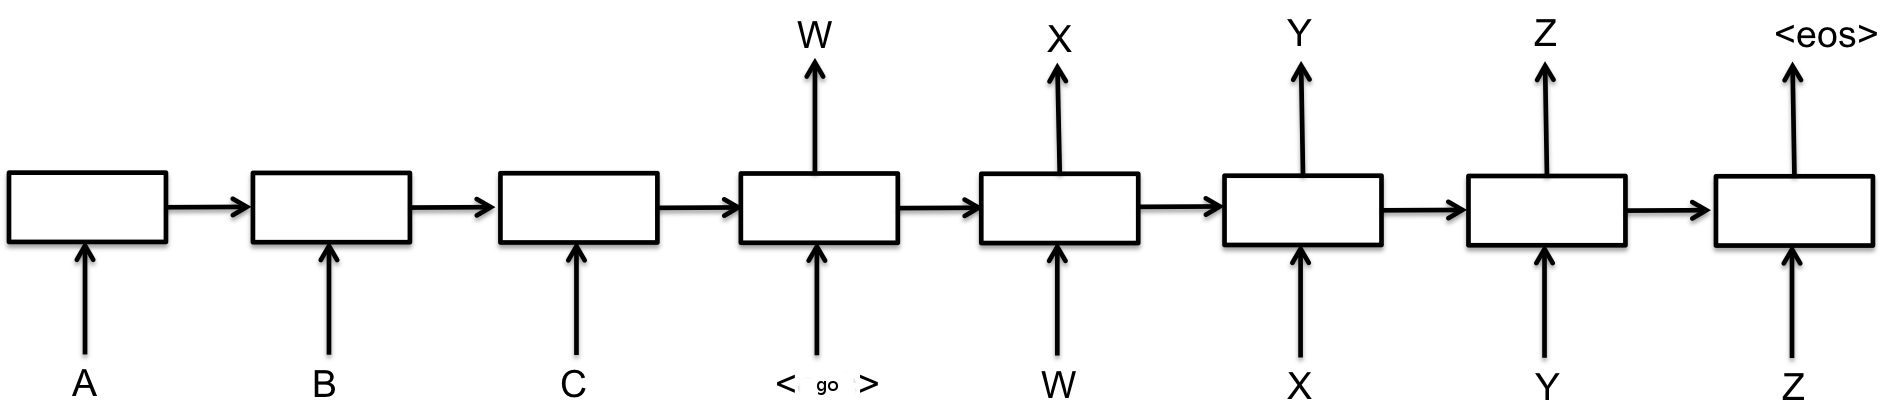
\includegraphics[width=\textwidth]{imgs/basic_seq2seq.png}
	\label{fig:seq2seq-basic}
	\centering
\end{figure}


Пусть входному предложению $\mathbf{x}$ соответствует ответ из выборки $y = \lbrace y_1, y_2, \dots, y_m\rbrace$. Ему соответствует последовательность векторных представлений $\mathbf{y} = \lbrace \mathbf{y_1}, \mathbf{y_2}, \dots, \mathbf{y_m} \rbrace$.

Скрытое состояние $\mathbf{h^{\text{dec}}_0}$ декодировщика инициализируется финальным скрытым состоянием кодировщика, то есть $\mathbf{h^{\text{dec}}_0} = \mathbf{h^{\text{enc}}_n}$.
Процесс генерации ответа выглядит следующим образом: вначале декодировщик принимает на вход служебный токен $\textbf{BOS}$ (точнее его векторное представление) и генерирует первое слово $\hat{y}_1$, семплируя из распределения $\hat{p}_1 = \text{softmax}(U\mathbf{h^{\text{dec}}_1})$. Затем векторное представление $\mathbf{\hat{y}_1}$ этого слова подается в качестве входа на следующем шаге, генерируется следующее слово и так далее. Процесс продолжается до тех пор, пока модель не сгенерирует служебный токен \textbf{EOS}. Для того, чтобы это случилось, на этапе обучения этот токен добавляется ко всем ответам в конец.

Однако, процесс обучения модели отличается от вышеописанного процесса генерации. На $t$-ом шаге генерации на вход сети подается векторное представление $(t-1)$-го слова из \textbf{правильного} ответа, то есть $\mathbf{y_{t-1}}$, а не слово, сгенерированное моделью на предыдущем шаге, как в случае с процессом генерации.

Формально, на этапе обучения модель моделирует факторизацию распределения ''языковой модели'':

\begin{equation} \label{eq:seq2seq-pdistr-train}
p(y | x) = p(y_1 | x) p(y_2 | y_1, x) \cdot \dots \cdot p(y_m | y_1, y_2, \dots, y_{m-1}, x)
\end{equation}

С помощью следующего параметризованного распределения:

\begin{equation} \label{eq:seq2seq-pdistr-train-2}
p_{\theta}(y_t | y_1, y_2, \dots, y_{t-1}, x) \approx p(y_t|y_1, y_2, \dots, y_{t-1}, x),
\end{equation}

где $\theta$ -- все параметры диалоговой модели. В то же время, на этапе тестирования, распределение выглядит иначе:

\begin{equation} \label{eq:seq2seq-pdistr-test}
p_{\theta}(y_t | \hat{y}_1, \hat{y}_2, \dots, \hat{y}_{t-1}, x)
\end{equation}

Эта разница между распределениями является известной проблемой, называющейся \textbf{несходством распределений} (англ. distribution discrepancy) и один из методов её решения предложен в статье \cite{DBLP:journals/corr/BengioVJS15}. Тем не менее, это не является большой проблемой для данной работы, но стоит заметить, что методы обучения с подкреплением неявно обходят эту проблему, так как оптимизируют модель используя \textbf{сгенерированные} ей ответы, а не правильные ответы из обучающей выборки.

Опишем функцию потерь на одном примере $(x, y)$ для обучения диалоговой модели:

\begin{equation} \label{crossentropy}
L(\theta) =  -\frac{1}{m}\sum_{t=1}^{m} \log\hat{p}_{ty_t} \xrightarrow[\theta]{} \min,
\end{equation}
где $|V|$ -- размер словаря, $m$ -- длина последовательности, а $\hat{p}_{ty_t}$ -- вероятность слова $y_t$ на шаге $t$. Эта функция потерь -- кроссэнтропия между распределениями $p_{\theta}(y_t | y_1, y_2, \dots, y_{t-1}, x)$ и $p(y_t|y_1, y_2, \dots, y_{t-1}, x)$.

На этапе тестирования модели, ответ генерируется жадным образом. На каждом шаге декодирование выбирается слово с максимальной вероятностью. Существуют улучшения данного метода, такие как beam-search (\cite{DBLP:journals/corr/abs-0907-0809}).

\pagebreak
\section{Обучение с подкреплением}

В этой главе описываются основы обучения с подкреплением, а также необходимый для дальнейшего понимания материал о policy-gradient методах.

\subsection{Введение в обучение с подкреплением}

Обучение с подкреплением -- класс методов для построения т.н. \textbf{агентов}, сущностей, взаимодействующих со \textbf{средой}. Агент может ''чувствовать'' среду (учитывать \textbf{состояния} среды) и действовать в ней. Целью агента является выбор оптимальных действий для достижения цели. Обучение с подкреплением отличается от классического машинного обучения, где присутствует выборка с правильными (оптимальными) ответами. Вместо этого, агенту необходимо исследовать среду методом проб и ошибок и понимать, как действовать в различных ситуациях. Например, на роботе установлены различные сенсоры в виде камер и дальномеров, с помощью которых он получает состояние среды, при этом робот может выбирать, в какую сторону ему двигаться. За каждое действие агент получает награду, таким образом понимая, что ''хорошо'' и что ''плохо''. Задачей агента является выучить \textbf{стратегию} выбора оптимальных действий в долгосрочной перспективе для достижения цели. Для этого агент поддерживает \textbf{кумулятивную награду} каждого состояния или каждой пары состояние-действие.

Обучение с подкреплением отличается от классического машинного обучения двумя свойствами:

\begin{enumerate}
	\item \textbf{Метод проб и ошибок.} Агент пробует различные действия в одном и том же состоянии, чтобы понять, какое из них ведёт к наибольшей кумулятивной награде. В классическом машинном обучении оптимальные метки даны сразу.
	\item \textbf{Запаздывающая награда.} Выполненные агентом действия влияют не только на награду, полученную в этот момент времени, но и на награды в будущем. В классическом машинном обучении предполагается, что все объекты выборки независимы.
\end{enumerate}

Завершая введение, агент в обучении с подкреплением использует свой собственный прошлый опыт взаимодействия со средой, чтобы улучшить свою стратегию в долгосрочной перспективе.

\subsection{Марковский процесс принятия решений}


Назовем \textbf{средой} марковский процесс принятия решений $\mathcal{M} = (\mathcal{S}, \mathcal{A}, P, r, \gamma)$, где $\mathcal{S}$ -- множество (возможно бесконечное) состояний, $\mathcal{A}$ -- множество (возможно бесконечное) допустимых действий агента, $P = P(s' | s,a)$ -- динамика среды, $r = r(s' | s, a)$ -- награда при совершении агентом действия $a$ и переходе среды из состояния $s$ в $s'$, $\gamma \in [0, 1]$ -- фактор дисконтирования. Вероятность $P(s' | s,a)$ есть вероятность среды перейти в состояние $s'$ при условии, что до этого она находилась в состоянии $s$ и агент совершил действие $a$. Фактор дисконтирования $\gamma$ определяет значимость наград в будущем: награда со значением $r$, полученная на $k$ моментов времени позже, будет в $\gamma^{k-1}$ раз ''дешевле'', чем полученная немедленно.

Введём сущность \textbf{агента}. Агент взаимодействует со средой во времени. В каждый момент времени $t$ агент находится в состоянии $s_t$, совершает действие $a_t$, получает от среды награду $r_t$ и переходит в следующее состояние $s_{t+1}$. Задача агента -- максимизировать дисконтированную суммарную награду $G_0 = \sum_{i=0}^{T}\gamma^i r_i$. Введем обобщение суммарной награды $G_t = \sum_{i=t}^{T}\gamma^i r_i$. Выбор действия агент производит в соответствии с \textbf{политикой} -- распределением $\pi(a|s) : \mathcal{A} \times \mathcal{S} \rightarrow [0, 1]$.

Общее представление о взаимодействии агента со средой представлено на Рис. \ref{fig:rl-overview}

\begin{figure}[htbp!]
	\caption{Взаимодействие агента со средой.}
	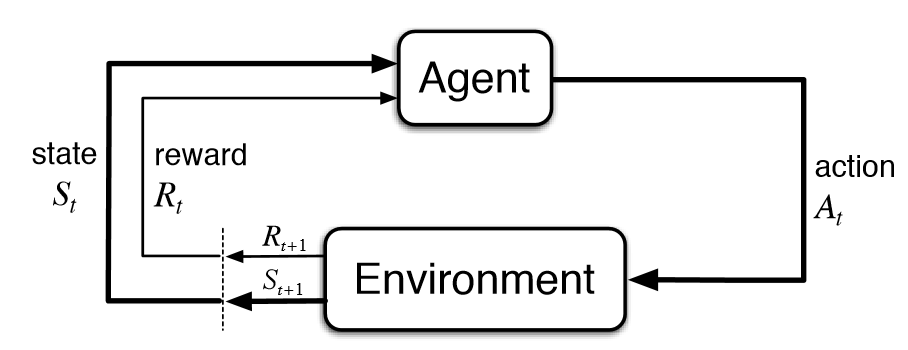
\includegraphics[width=\textwidth]{imgs/rl_overview2.png}
	\label{fig:rl-overview}
	\centering
\end{figure}

Важным предположением во всём обучении с подкреплением является \textbf{гипотеза о марковости среды}:

\begin{equation} \label{eq:rl-markov-property}
p(s_{t+1}, r_{t+1}|s_0, a_0, r_1 \dots, s_{t-1}, a_{t-1}, r_t, s_t, a_t) = p(s_{t+1}, r_{t+1} | s_t, a_t)
\end{equation}

Это свойство позволяет предсказать следующее состояние, имея текущее состояние и совершенное агентом действие. Большинство доказательств алгоритмов обучения с подкреплением используют это свойство. В действительности агент не имеет доступа к истинному состоянию среды, которое обладает свойством марковости. Агент лишь получает \textit{наблюдения} от среды, тем самым обновляя своё состояние $s$. Справедливости ради, стоит заметить, что в большинстве случаев можно добиться того, что условие марковости для состояния агента будет ''почти'' выполнятся и на практике алгоритмы будут работать.

На Рис. \ref{fig:mdp} показана иллюстрация к марковскому процессу принятия решений.

\begin{figure}[htbp!]
	\caption{Пример марковского процесса принятия решений.}
	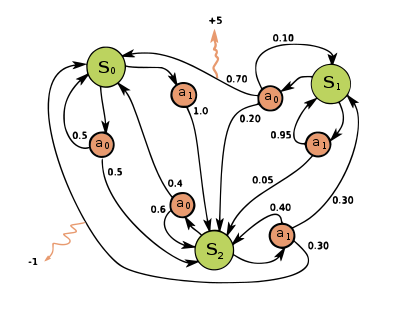
\includegraphics[scale=0.7]{imgs/mdp.png}
	\label{fig:mdp}
	\centering
\end{figure}


\subsection{Функции полезности состояния. Уравнения Беллмана}

Почти все алгоритмы обучения с подкреплением включают в себя оценку т. н. \textbf{функций полезности} -- функций, которые принимают на вход состояние и выдают оценку того, насколько агенту выгодно находится в этом состоянии (или принимают на вход пару состояние-действие, на выходе оценка того, насколько выгодно агенту совершить действие в данном состоянии).

Формально, определим \textbf{функцию полезности состояния} для политики $\pi(a|s)$:

\begin{equation} \label{eq:rl-value-function}
v_{\pi}(s) \doteq \mathbb{E}_{\pi}\lbrack G_t | S_t = s\rbrack = \mathbb{E}_{\pi}\bigg[\sum_{k=0}^{\infty}  \gamma^k R_{t+k+1} \bigg| S_t = s \bigg]
\end{equation}

В правой части стоит ожидаемая кумулятивная награда, если агент действует согласно политике $\pi$ из состояния $s$.

Аналогично, определим \textbf{функцию полезности состояния-действия}:

\begin{equation} \label{eq:rl-qvalue-function}
q_{\pi}(s, a) \doteq \mathbb{E}_{\pi}\lbrack G_t | S_t = s,~ A_t = a\rbrack = \mathbb{E}_{\pi}\bigg[\sum_{k=0}^{\infty}  \gamma^k R_{t+k+1} \bigg| S_t = s,~ A_t = a\bigg]
\end{equation}

Фундаментальным свойством, используемым повсюду в обучении с подкреплением, является тот факт (\cite{sutton1998reinforcement}), что они удовлетворяют следующим рекуррентным соотношениям, называющимися \textbf{уравнениями Беллмана}:

\begin{align}
v_{\pi}(s) &= \sum_a \pi(a | s) \sum_{s'} p(s' | s, a) \lbrack r(s' | s, a) + \gamma v_{\pi}(s') \rbrack, \label{eq:rl-bellman-equations-1} \\
q_{\pi}(s, a) &= \sum_{s'} p(s' | s, a) \lbrack r(s' | s, a) + \gamma v_{\pi}(s') \rbrack \label{eq:rl-bellman-equations-2}
\end{align}

Оптимальная стратегия $\pi^*$ может быть получена из \textbf{уравнений оптимальности Беллмана}:

\begin{align}
v^*(s) &= \max_{\pi} v_{\pi}(s) = \max_a \sum_{s'} p(s' | s, a) \lbrack r(s' | s, a) + \gamma v^*(s') \rbrack, \label{eq:rl-bellman-optimality-equations-1}\\
q^*(s, a) &= \max_{\pi} q_{\pi}(s, a) = \sum_{s'} p(s' | s, a) \lbrack r(s' | s, a) + \gamma \max_{a'}q^*(s', a') \rbrack \label{eq:rl-bellman-optimality-equations-2}
\end{align}

Тогда оптимальная стратегия есть $\pi^*(s) = \arg\max_a q^*(s, a)$.

Методы для поиска оптимальной политики, использующие уравнения \eqref{eq:rl-bellman-optimality-equations-1} и \eqref{eq:rl-bellman-optimality-equations-2}, принадлежат так называемому классу value-based методов обучения с подкреплением. Примеры: Q-learning, SARSA (\cite{sutton1998reinforcement}).

\subsection{Policy-gradient алгоритмы обучения с подкреплением}

В данном разделе рассматривается некая противоположность value-based подхода, а именно класс policy-based методов, идея которых заключается в параметризации стратегии и её оптимизации напрямую. Также, часто этот класс называют policy-gradient в связи с оптимизацией политики напрямую методом градиентного спуска.

Будем рассматривать параметризованные стохастические политики $\pi_{\theta}(a|s)$, $\theta \in \mathbb{R}^n$ и пытаться максимизировать кумулятивную награду $G_0$. \textbf{Функционалом полезности политики} назовем

\begin{equation} \label{eq:pg-performance-measure}
\eta(\theta) \doteq \mathbb{E}_{\pi_{\theta}}[G_0] = v_{\pi_{\theta}}(s_0)
\end{equation}


В ранних работах (\cite{sutton1998reinforcement}, \cite{sutton1999policy}) был установлен основной результат, позволяющий максимизировать \eqref{eq:pg-performance-measure}. Следуя ему, можно записать:

\begin{equation} \label{eq:pg-theorem-grad}
\nabla_\theta \eta = \mathbb{E}_{\pi_{\theta}} \nabla_\theta \log \pi_{\theta} (a | s) \cdot q_{\pi_{\theta}}(s)
\end{equation}

На практике матожидание в \eqref{eq:pg-theorem-grad} заменяется семплированием из текущей политики, а функция полезности $q_{\pi_{\theta}}(s)$ заменяется на её оценку.

Рассмотрим различные методы, получающиеся из \eqref{eq:pg-theorem-grad}.

\subsubsection*{\textbf{REINFORCE}}

Так как $G_t$ является несмещённой оценкой $q_{\pi_{\theta}}(s)$, то производя замену, получаем метод REINFORCE: $\Delta \theta = \sum_{t} \nabla_\theta \log \pi_{\theta} (a_t | s_t) \cdot G_t$.

\subsubsection*{\textbf{REINFORCE with baseline}}

На практике часто бывает, что $G_t$ имеет большую дисперсию. Показано (\cite{sutton1998reinforcement}, \cite{sutton1999policy}), что $\sum_{t}\nabla_\theta \log\pi_{\theta}(a_t|s_t) \cdot (G_t - b(s_t)) $ также является градиентом функционала полезности политики. Такой метод называется REINFORCE with baseline. Добавка $b(s)$, называемая бейзлайном, позволяет уменьшить дисперсию оценки функции полезности при обучении и не влияет на градиент \eqref{eq:pg-theorem-grad}.

\subsubsection*{\textbf{Actor-Critic}}

В качестве бейзлайна можно взять параметризованную $v_\pi$, которая будет обучаться вместо с политикой согласно Q-learning обновлениям. Таким образом, получаем метод Actor-Critic и формулу обновления весов $\Delta \theta = \sum_t (G_t - v(s_t)) \nabla_\theta\log\pi_{\theta}(a_t|s_t)$.

\subsubsection*{\textbf{Advantage Actor-Critic}}

Метод Advantage Actor-Critic (A2C) также использует факт, что $r_{t+1} + \gamma v_\pi(s_{t+1})$ также является несмещенной оценкой $q_\pi(s_t, a_t)$ (следует из \eqref{eq:rl-bellman-equations-2}). Метод Actor-Critic комбинирует value-based и policy-based подходы. Формула обновления выглядит следующим образом: $\Delta \theta = \sum_t (r_{t+1} + \gamma v(s_{t+1})  - v(s_t)) \nabla_\theta\log\pi_{\theta}(a_t|s_t)$.

\subsection{Обучение с подкреплением в нейросетевых диалоговых моделях}

В нейросетевой диалоговой модели естественно принять распределение на словах $\hat{p}_t$ в качестве политики. Параметрами политики будут все параметры диалоговой модели. Также можно параметризовать политику лишь параметрами декодировщика, а кодировщик оставлять неизменным.

В такой постановке, действиями будут являться генерируемые декодировщиком слова, а состояниями агента -- вектора скрытых состояний $\mathbf{h_t}$. Таким образом, можно задавать различные функции наград за генерируемые слова и дообучать модель одним из вышеперечисленных методов.

\pagebreak
\section{Обзор литературы}

\subsubsection*{\textbf{A Persona-Based Neural Conversational Model}}

Основная работа, пытающаяся решить задачу консистентности спикера. Основная идея заключается в обуславливании декодировщика не только на контекст предложения, но и на векторное представление пользователя. Векторное представление подается в ячейку рекуррентной сети на каждом шаге декодирования ответа и выучивается вместе с сетью на обучающей выборке. Архитектура нейронной сети представлена на Рис. \ref{fig:persona-based}.

\begin{figure}[htbp!]
	\caption{Архитектура Persona-based Conversational Model.}
	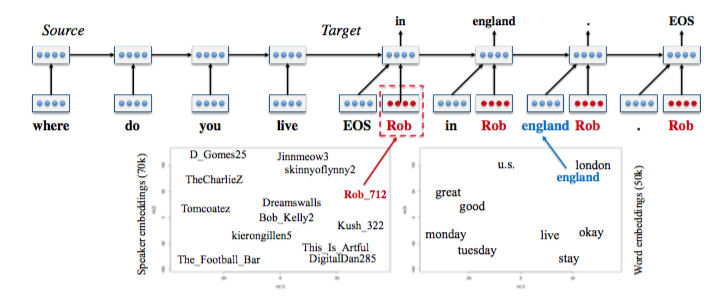
\includegraphics[scale=0.7]{imgs/persona-based.png}
	\label{fig:persona-based}
	\centering
\end{figure}

Отличие эксперимента \textbf{BeLikeX} в настоящей работе в исследовании применимости обучения с подкреплением для данной задачи, а также скорости сходимости обучения.


\subsubsection*{\textbf{Deep Reinforcement Learning for Dialogue Generation}}

Работа не имеет прямого отношения к настоящей, но интересна своим подходом к решению основных проблем нейросетевых диалоговых моделей, таких как:

\begin{itemize}
	\item \textbf{Общие ответы.} Реплики "я не знаю", "без понятия", "не понимаю о чем вы говорите" и т.п. имеют обладают высокой вероятностью по языковой модели, из-за чего модель генерирует их на большое множество контекстов.
	\item \textbf{Зацикливание модели.} Если модель запустить в режиме разговора самой с собой, то она быстро зацикливается, чередуя две реплики друг с другом. Это происходит из-за отсутствия новой информации в ответе модели. Авторы стремятся увеличить поток информации в ответах модели на каждом шаге диалога.
\end{itemize}

Авторская попытка решить эти проблемы заключается во введении трёх функций наград за сгенерированные моделью ответы. Дообучение происходит с помощью policy-gradient метода REINFORCE.

Качественное сравнение авторской модели с бейзлайном можно видеть на Рис. \ref{fig:rl-dialog-generation-paper}.

\begin{figure}[htbp!]
	\caption{Ответы бейзлайна и модели из статьи DRL for Dialogue Generation.}
	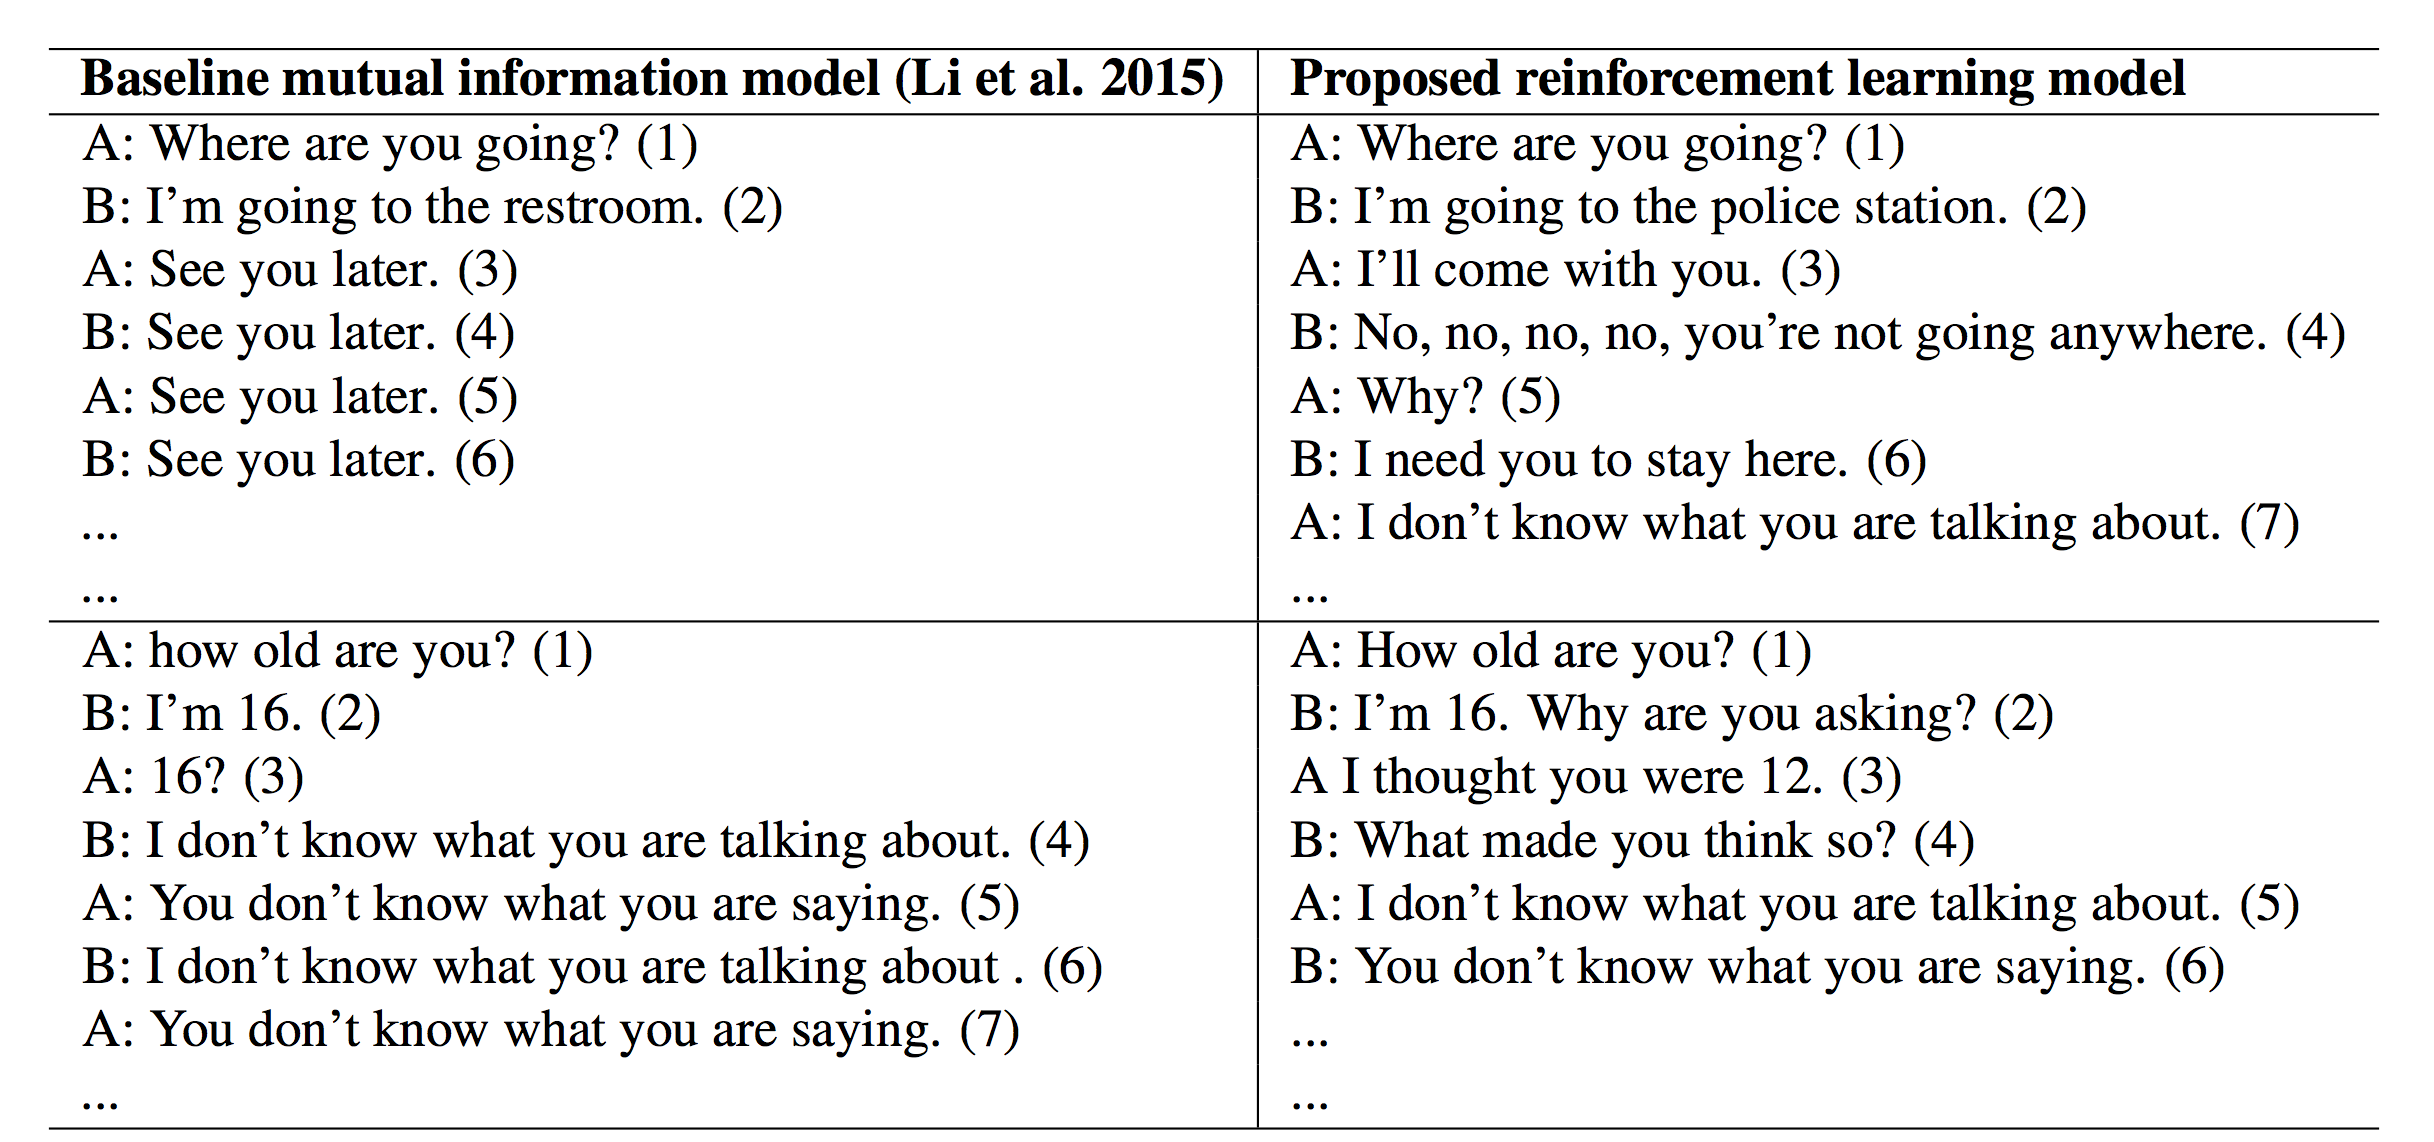
\includegraphics[width=\textwidth]{imgs/rl-dialog-generation-paper.png}
	\label{fig:rl-dialog-generation-paper}
	\centering
\end{figure}


\subsubsection*{\textbf{Sample-efficient Deep Reinforcement Learning for Dialog Control}}

Основной целью статьи является уменьшение необходимого количества объектов в обучающей выборке для обучения целеориентированной диалоговой системы. Авторы исследуют методы REINFORCE, REINFORCE with baseline, Actor-Critic применительно к этой задаче, а также демонстрируют пользу техники Experience Replay (\cite{DBLP:journals/corr/MnihKSGAWR13}).

\subsubsection*{\textbf{Hybrid Code Networks}}

Авторы демонстрируют нейросетевую архитектуру для целеориентированных диалоговых систем, которая позволяет интегрировать компоненты, написанные разработчиком, напрямую в нейросеть. Также авторы показывают, как дообучать такую систему с помощью обучения с подкреплением в online-режиме. Архитектура сети представлена на Рис. \ref{fig:hcn}.

\begin{figure}[htbp!]
	\caption{Архитектура из статьи Hybric Code Networks.}
	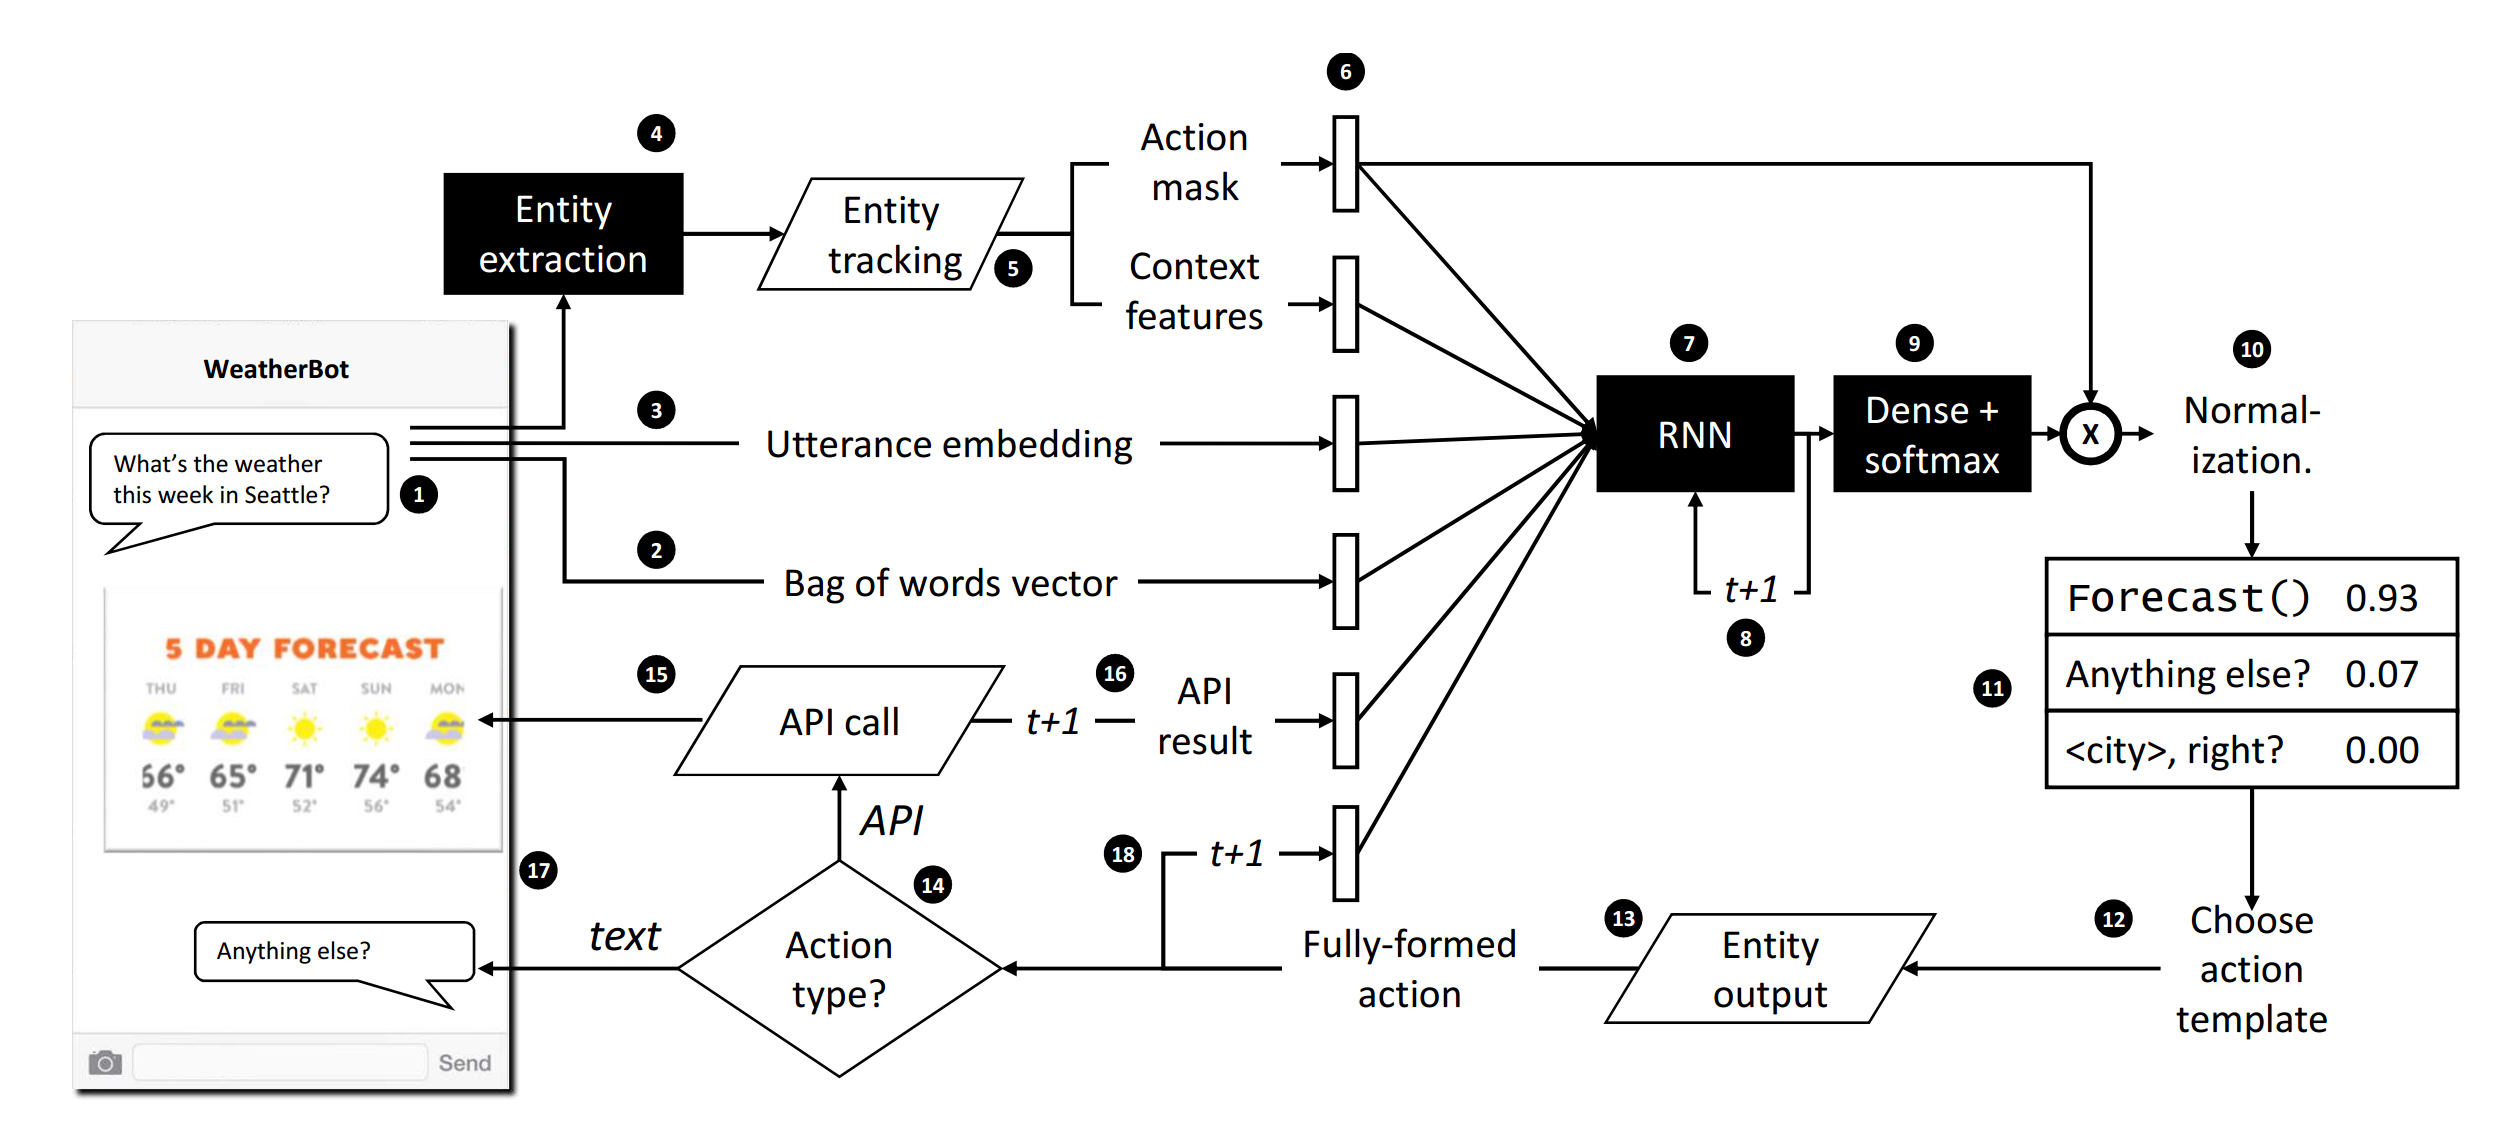
\includegraphics[width=\textwidth]{imgs/hcn.png}
	\label{fig:hcn}
	\centering
\end{figure}


\subsubsection*{\textbf{Self-critical Sequence Training for Image Captioning}}

В данной статье вводится принципиально новый policy-gradient алгоритм, называющийся \textbf{Self-critical Sequence Training} (SCST). Авторы проводят эксперименты на задаче описания изображений, используя классический датасет MSCOCO (\cite{DBLP:journals/corr/LinMBHPRDZ14}), и устанавливают лучший результат в сравнении с прошлыми работами.

Алгоритм напрямую оптимизирует целевую метрику CIDEr, по которой измеряется качество модели на тестовой выборке. Рассмотрим этот подход, так как именно он будет использоваться в эксперименте \textbf{BeLikeX}.

На этапе тестирования последовательность слов генерируется жадным образом. Таким образом, сгенерированный ответ зависит только от начального состояния декодировщика $\mathbf{h^{\text{dec}}_0}$. Это позволяет использовать значение метрики на таком ответе в качестве бейзлайна в алгоритме REINFORCE with baseline. Таким образом, обновление весов происходит по следующей схеме:

\begin{equation} \label{eq:rl-scst}
\Delta \theta = \nabla_\theta \log p_{\theta}(\hat{y}_1, \hat{y}_2, \dots, \hat{y}_m | \mathbf{h^{\text{dec}}_0}) \cdot (r(\hat{y}_1, \hat{y}_2, \dots, \hat{y}_m) - r(\overline{y}_1, \overline{y}_2, \dots, \overline{y}_m)),
\end{equation}

где $\hat{y}_t$ -- $t$-ое слово ответа, сгенерированного семплированием, $\overline{y}_t$ -- $t$-ое слово ''жадного'' ответа, $r(y)$ -- функция награды (в статье используется CIDEr).


\pagebreak
\section{Эксперимент BePolite}

\subsection{Постановка задачи}

Целью данного эксперимента является уменьшение обсценной лексики в ответах диалоговой модели. При этом требуется сохранить грамматическую и смысловую структуры ответа.

Обозначим обучающую выборку пар контекст-ответ как $\mathcal{D} = \lbrace (x^{(i)}, y^{(i)}) \rbrace_{i=1}^N$, а множество обсценных слов как $\mathcal{S} = \{w_1, w_2, \dots, w_M\}$. Также обозначим диалоговую модель с набором параметров $\theta$ как $G_\theta (x) \rightarrow \hat{y}$. 

Введём функцию награды за сгенерированное слово $r(\hat{y}_t) = -\mathbb{I}(\hat{y}_t \in \mathcal{S})$. Тогда кумулятивная награда за сгенерированный ответ есть $R(\hat{y}) = \sum_{t=1}^m r(\hat{y}_t)$.

Теперь можно записать функционал потерь на одном примере обучающей выборки:

\begin{equation} \label{eq:rl-bepolite-loss}
GL(\theta) = \mathbb{E}_{x,y \sim \mathcal{D}}\big[\alpha\sum_{t} \log p_\theta (y_t | y_1, y_2, \dots, y_{t-1}, x) + R(G_\theta(x))\big] \xrightarrow[\theta]{} \max
\end{equation}

В реализации матожидание оценивается через среднее по обучающей выборке.

Заметим, что функция $R(\hat{y})$ недифференцируема по параметрам сети $\theta$, но обучение с подкреплением позволяет обойти эту проблему. Число $\alpha$ есть вес ''классического'' кроссэнтропийного функционала потерь.

\subsection{Входные данные}

Обучающей выборкой являются субтритры к англоязычным фильмам с сайта \url{opensubtitles.org}. Размер обучеющей выборки составляет 18 миллионов пар контекст-ответ. Размер валидационной -- 100 тысяч пар. Длина контекста равна двум репликам. Примеры обучающих пар можно видеть в Табл. \ref{table:opensub-data}.

Размер словаря с обсценной лексикой составил ~500 слов.

\begin{center}
\begin{table}[htbp]
\caption{Примеры обучающих фраз из датасета \textit{opensubtitles}.}
\label{table:opensub-data}
\begin{tabulary}{\textwidth}{|L|L|}
	\hline
	Контекст & Ответ \\
	\hline \hline
	Hey, do we know anyone who has strawberry milk? \textbf{EOS} Yeah, I think Donnie's got some. \textbf{EOS} & \textbf{BOS} Donnie Freckles? \textbf{EOS} \\
	\hline
	Is it true that you have a magic ring that can make you invisible? \textbf{EOS} Uh, yeah. \textbf{EOS} & \textbf{BOS} That is so cool! Hey, I just thought of something. \textbf{EOS} \\
	\hline
	I need you to start catching for me. \textbf{EOS} What? \textbf{EOS} & \textbf{BOS} Yeah, I need you to be my catcher, at least until \textbf{EOS} \\
	\hline 
	Can I help you? \textbf{EOS} We want to play the winners. The losers of this game are playing the winners. \textbf{EOS} & \textbf{BOS} But that is not fair. \textbf{EOS} \\
	\hline
	Do you really need a diploma? \textbf{EOS} Jeff learned how to print diplomas. \textbf{EOS} & \textbf{BOS} As well as the diplomacy and perseverance. \textbf{EOS} \\
	\hline
	Come here. \textbf{EOS} What is that, Alex? \textbf{EOS} & \textbf{BOS} I don't know. \textbf{EOS} \\
	\hline 
\end{tabulary}
\end{table}
\end{center}


\subsection{Метрики качества}

Результат оценивается по двум метрикам на валидационной выборке:

\begin{enumerate}
	\item \textbf{Перплексия}. $\text{PPL} = \exp^{-\frac{1}{N}\sum_{i=1}^N \log p_\theta (y^{(i)} | x^{(i)})}$.
	\item \textbf{Средняя награда}. $\text{avgR} = \frac{1}{N}\sum_{i=1}^N R(G_\theta(x^{(i)}))$.
\end{enumerate}

Перплексия является стандартной метрикой для оценки языковых моделей. Вторая метрика -- среднее количество обсценных слов в ответах модели.

\subsection{Базовое решение}

В качестве диалоговой модели была обучена 1-слойная LSTM сеть с размером скрытого слоя 1024. Размер словаря составил 50000 наиболее частотных слов. Последнее состояние кодировщика использовалось не только для инициализации декодировщика, но и подавалось в него на каждом шаге декодирования. Размерность векторных представлений 500, представления обучались вместе с сетью. Обучение длилось, пока значение функционала потерь падало на валидационной выборке (около 4 суток).

\subsection{Решение}

В качестве основного подхода к дообучению модели был выбран метод Advantade Actor-Critic (A2C). Модель, аппроксимирующая функцию полезности состояния, принимает на вход скрытое состояние декодировщика на каждом шаге, пропускает его через два полносвязных слоя по 512 нейронов, затем через слой в 256 нейронов. Функция активации -- ReLu. Наконец, линейная комбинация из 256 нейронов используется как оценка value-function. Архитектура отображена на Рис. \ref{fig:critic}.

\begin{figure}[htbp!]
	\caption{Архитектура ''критика'' в эксперименте BePolite.}
	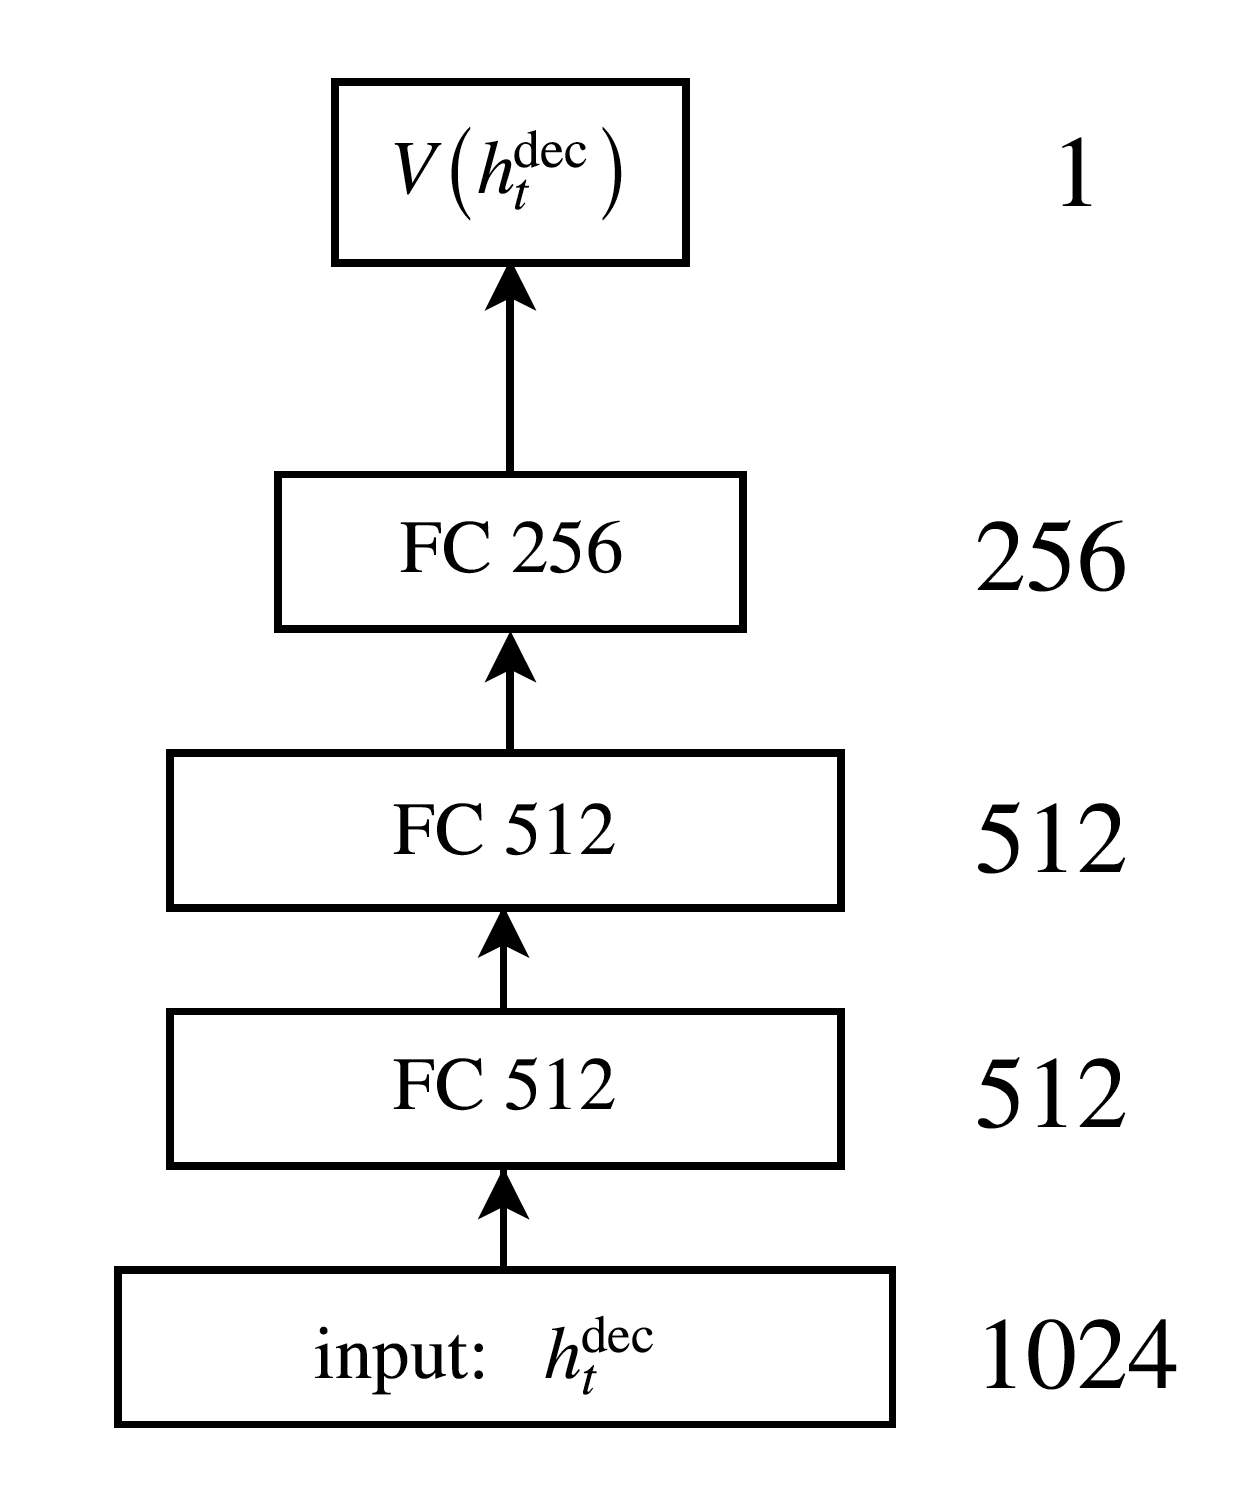
\includegraphics[scale=0.5]{imgs/critic.png}
	\label{fig:critic}
	\centering
\end{figure}

Дообучение происходило на той же обучающей выборке, на 32000 случайных примерах.

\subsection{Результаты}

В Табл. \ref{table:bepolite-baseline} представлены значения метрик для базовой модели.

\begingroup
\renewcommand{\arraystretch}{1.8}
\begin{center}
	\begin{table}[htbp]
		\caption{Значения метрик для базовой модели.}
		\label{table:bepolite-baseline}
		\begin{tabular}{|c|c|}
			\hline
			\textbf{PPL} & \textbf{avgR} \\ 
			\hline
			3.142 & -0.136 \\
			\hline
		\end{tabular}
	\end{table}
\end{center}
\endgroup

В Табл. \ref{table:bepolite-results} показаны результаты модели после дообучения по методу A2C для разных значений $\alpha$.

\begingroup
\renewcommand{\arraystretch}{1.8}
\begin{table}[htbp!]
	\centering
	\begin{tabular}{|l|c|c|}
		\hline
		$\alpha$ & \textbf{PPL}                   &    \textbf{avgR} \\
		\hline 
		5 &  3.297 & -0.021 \\ 
		\hline
		20 & 3.270 & -0.065 \\
		\hline 
	\end{tabular}
	\caption{Значения метрик A2C модели.}
	\label{table:bepolite-results}
\end{table}
\endgroup

Таким образом, наблюдается снижение обсценной лексики в 6-7 раз. Базовая модель генерирует в среднем 130 обсценных слов на 1000 ответов, а модель дообученная по методу A2C всего 20 слов на 1000 ответов. При этом значения перплексии ухудшаются незначительно.


\pagebreak
\section{Эксперимент BeLikeX}

Цель данного эксперимента -- заставить модель генерировать ответы, похожие на ответы какой-либо персоны.

\subsection{Постановка задачи}

Опять, обозначим обучающую выборку пар контекст-ответ как $\mathcal{D} = \lbrace (x^{(i)}, y^{(i)}) \rbrace_{i=1}^N$, а диалоговую модель с набором параметров $\theta$ как $G_\theta (x) \rightarrow \hat{y}$. 

Пусть $D_{\text{uid}}(y) \rightarrow [-1, 1],$ -- функция, принимающая на вход предложение (вектор натуральных чисел) $y$ и выдающая ''меру похожести'' предложения $y$ на типичный ответ пользователем $\text{uid}$. Будем считать эту функцию наградой за генерацию ответа $y$ моделью $G_\theta$. Конкретная реализация данной функции будет приведена ниже.

Эта функция наград никак не учитывает контекст, получаемый на вход моделью, поэтому, если максимизировать только её, модель может выродиться и генерировать один и тот же ответ пользователя на все контексты. В связи с этим, в функционал потерь необходимо добавить функционал от языковой модели, аналогично \eqref{eq:rl-bepolite-loss}.

Теперь можно записать оптимизационную задачу:

\begin{equation} \label{eq:rl-belikex-loss}
GL(\theta) = \mathbb{E}_{x,y \sim \mathcal{D}}\big[\alpha\sum_{t} \log p_\theta (y_t | y_1, y_2, \dots, y_{t-1}, x) + D_{\text{uid}}(G_\theta(x))\big] \xrightarrow[\theta]{} \max.
\end{equation}

В реализации матожидание оценивается через среднее по обучающей выборке. Число $\alpha$ играет ту же роль, что и в эксперименте BePolite.

\subsection{Входные данные}

Опишем данные, использовавшиеся в эксперименте:

\begin{enumerate}
	\item Выборка $ \mathcal{D}_g $. Данные из русскоязычной социальной сети Twitter. Объем -- 50 миллионов пар контекст-ответ. Необходима для обучения базовой диалоговой модели. Объём валидационной выборки -- 100 тысяч примеров. Примеры диалогов представлены в Табл. \ref{table:belikex-twitter-general}.
	\item Выборка $ \mathcal{D}_u $. Получена из отдельной выборки из Twitter'а, в которой к каждому сообщению привязан идентификатор пользователя, путём отбора пар контекст-ответ, ответ в которых принадлежит одному из 1000 пользователей с наибольшими количествами ответов. Объём -- 1,2 миллиона обучающих примеров. Необходима для обучения модели, соответствующей функции похожести. Архитектура модели описана ниже.
	\item Выборка $\mathcal{D}_s$. Получена из $\mathcal{D}_u$ путём отбора реплик, принадлежащих пользователю, который был идентифицирован как техническая поддержка сотового оператора. Объём -- 3000 обучающих примеров (500 примеров в валидационной выборке). Примеры диалогов представлены в Табл. \ref{table:belikex-twitter-support}.
\end{enumerate}

\begin{center}
	\begin{table}[htbp]
		\caption{Примеры обучающих фраз из выборки $ \mathcal{D}_g $.}
		\label{table:belikex-twitter-general}
		\begin{tabulary}{\textwidth}{|L|L|}
			\hline
			Контекст & Ответ \\
			\hline \hline
			Слава инстаграму, героям iii слава! Не забывай про геймеров. \textbf{EOS} Поизвращаемся - героям 4 (!!!) слава. \textbf{EOS} & \textbf{BOS} Матерь божья!  \textbf{EOS} \\
			\hline
			Я тоже самое маме сказал \textbf{EOS} Брат по несчастью. \textbf{EOS} & \textbf{BOS} Я не про свой город сказал. Прости :с \textbf{EOS} \\
			\hline
			Я ринусь в бой, достойный схватки, последней на мой век. Живи и умирай в сей день. Живи...и умирай...в сей день. \textbf{EOS} Особенно печальный момент, когда он бумажники все в стопочку складывает и вспоминает свою семью... Ах. Я рыдала \textbf{EOS} & \textbf{BOS} Да. Я тоже! Весь фильм со слезами на глазах... до сих пор не отошла, все думаю, как бы я поступила... смогла бы...? \textbf{EOS} \\
			\hline 
			точно не скоро:3 \textbf{EOS} ахах это почему? :d \textbf{EOS} & \textbf{BOS} сериалыыыы:3 \textbf{EOS} \\
			\hline
			Так блин это фильм а это сериалы:d \textbf{EOS} Все равно ты непостоянная смирись \textbf{EOS} & \textbf{BOS} ахахаа лол \textbf{EOS} \\
			\hline
			Родители смотрят рождественские встречи с пугачевой а я ржу ибо вспоминаю ту упоротость со стайлсом и пугачевой \textbf{EOS} По первому, да ? Сочувствую, мои тоже \textbf{EOS} & \textbf{BOS} Я с украины и у меня по интеру идет. Вообщем аля первый только в украине \textbf{EOS} \\
			\hline 
		\end{tabulary}
	\end{table}
\end{center}

\begin{center}
	\begin{table}[!hbtp]
		\caption{Примеры обучающих фраз из выборки $ \mathcal{D}_s $.}
		\label{table:belikex-twitter-support}
		\begin{tabulary}{\textwidth}{|L|L|}
			\hline
			Контекст & Ответ \\
			\hline \hline
			Жаль, что с я связан корпоративным тарифом. Очень хочется перейти на оператора с нормальным покрытием. \textbf{EOS} и мегафон здесь не берёт, и папа джонс не везёт пиццу \textbf{EOS} & \textbf{BOS} Добрый вечер! Укажите, пожалуйста, точный адрес (нас. пункт, улицу, номер дома), в чем именно заключается сложность. Проверим. \textbf{EOS} \\
			\hline
			на модем который используется как роутер списаны звонки, и всякое такое чего у меня в тарифе нету... \textbf{EOS} сервис на высшем уровне! Такое сейчас время, не своруешь не проживёшь , жаль ! Хорошая была компания! \textbf{EOS} & \textbf{BOS} коллеги, обратите внимание. \textbf{EOS} \\
			\hline
			Добрый вечер! С какими сложностями Вы столкнулись, скажите, пожалуйста? Постараемся Вам помочь. \textbf{EOS} интернет работал только "Е" полтора часа,уже все хорошо. \textbf{EOS} & \textbf{BOS} Рады, что Ваш вопрос решился. Возникнут вопросы - обращайтесь! =\text{)} \textbf{EOS} \\
			\hline 
			Добрый день! Для получения корректного ответа от специалиста уточните свой регион. \textbf{EOS} мурманская область \textbf{EOS} & \textbf{BOS} Коллеги, просьба проверить. \textbf{EOS} \\
			\hline
			Добрый день! Если сложности еще сохраняются, пожалуйста, уточните Ваш регион. \textbf{EOS} эти сложности были в начале Тверской в период массового скопления граждан. \textbf{EOS} & \textbf{BOS} Если есть такая возможность, то уточните, пожалуйста, адрес более подробно - для проверки требуются название улицы и номер дома.\textbf{EOS} \\
			\hline
			Без согласия Абонента услуга не отключается. \textbf{EOS} Зато без согласия абонента услуга подключается. \textbf{EOS} & \textbf{BOS} Платные услуги подключаются либо самим абонентом, либо сотрудником компании с согласия абонента. \textbf{EOS} \\
			\hline 
			здравствуйте! Это платный контент. Для отключения введите команду на своем телефонном аппарате. \textbf{EOS} Сейчас буду разбираться, подключилась или нет "в тихую" эта платная дрянь. \textbf{EOS} & \textbf{BOS} просьба обратить внимание . \textbf{EOS} \\
			\hline
			какой у Вас регион? \textbf{EOS} Пермь \textbf{EOS} & \textbf{BOS} Коллеги просьба проверить \textbf{EOS} \\
			\hline
			здравствуйте! Уточните, пожалуйста, по какому адресу наблюдаются сложности с интернетом \textbf{EOS} по всему городу Томску. Фрунзе 120, Лазо 24, Мира 35. Проблема не локальная и не частная. \textbf{EOS} & \textbf{BOS} Коллеги обратите, пожалуйста, внимание \textbf{EOS} \\
			\hline
			более чем. Dial up быстрее. \textbf{EOS} это вот мегафон у меня так работает( беда-беда огорчение \textbf{EOS} & \textbf{BOS} Добрый вечер. Какой у Вас регион? \textbf{EOS} \\
			\hline
			Позвонил в Рязанский Россельхозбанк. Так приятно никогда не общался с поддержкой. Всякие мегафоны отдыхают в стороне \textbf{EOS} ты общался с техподдержкой мегафона?? ОНА СУЩЕСТВУЕТ??! \textbf{EOS} & \textbf{BOS} Обратите, пожалуйста, внимание \textbf{EOS} \\
			
 		\end{tabulary}
	\end{table}
\end{center}


\subsection{Метрики качества}

Перечислим метрики, по которым будем оценивать качество решения:

\begin{enumerate}
	\item \textbf{Перплексия}. $\text{PPL} = \exp^{-\frac{1}{N}\sum_{i=1}^N \log p_\theta (y^{(i)} | x^{(i)})}$.
	\item \textbf{Средняя похожесть на пользователя}. $\text{avgD} = \frac{1}{N}\sum_{i=1}^N D_{\text{uid}}(G_\theta(x^{(i)}))$.
	\item \textbf{Человеческая оценка}. Будем смотреть на ответы разных моделей глазами.
\end{enumerate}


Аналогично эксперименту BePolite, дообучая модель по функционалу потерь, где присутствует не только слагаемое от языковой модели, значение перплексии будет неизменно ухудшаться. Но так как перплексия не является целевой метрикой задачи, то достаточно следить, что её значения остаются в пределах нормы.

Так как целевым пользователем была выбрана тех. поддержка, то целесообразно считать метрики на выборке $\mathcal{D}_s$ помимо $\mathcal{D}_g$.

\subsection{Базовое решение}

Базовое решение состоит из двух частей: диалоговой модели и реализации функции ''похожести'' $D(y)$. Опишем каждую из них.

\begin{itemize}
	\item \textbf{Диалоговая модель}. Диалоговая модель имеет такую же архитектуру, как модель из предыдущего эксперимента, только обучается на выборке $\mathcal{D}_g$. Словарь -- так же 50000 наиболее частотных слов в выборке $\mathcal{D}_g$. Обучение длилось около 7 суток.
	\item \textbf{Функция похожести}. Для реализации функции похожести была обучена модель из класса, часто называемый \textit{Deep Semantic Structured Model} или \textit{Deep Semantic Similarity Model} (\cite{semantic-parsing-for-single-relation-question-answering} \cite{learning-deep-structured-semantic-models-for-web-search-using-clickthrough-data} \cite{learning-continuous-phrase-representations-for-translation-modeling} \cite{learning-semantic-representations-using-convolutional-neural-networks-for-web-search} \cite{a-latent-semantic-model-with-convolutional-pooling-structure-for-information-retrieval}). Архитектура модели представлена на Рис. \ref{fig:belikex-dssm}. Модель состоит из двух ''башен''.
	
	Первая башня принимает на вход идентификатор пользователя $\text{uid}$ и отображает его в семантическое пространство пользователей-фраз посредством двух слоёв. Вначале действует эмбеддинг слой, отображающний идентификатор в его векторное представление размерности 128. Затем этот вектор проходит через полносвязный слой с 256 нейронами. Получившийся вектор $u$ и считается представлением пользователя в семантическом пространстве.
	
	Вторая башня принимает на вход предложение и пропускается через рекуррентный кодировщик с размером скрытого слоя 1024. Финальное скрытое состояние кодировщика проходит через полносвязный слой с 256 нейронами. Получившийся вектор $a$ интепретируется как представление фразы в семантическом пространстве.
	
	Мера похожести фразы $y$ на стиль пользователя $\text{uid}$ вычисляется как скалярное произведение соответствующих векторов в евклидовом пространстве. Во избежание слишком больших по модулю скалярных произведений, вектора $u$ и $a$ нормируются на сферу:
	
	\begin{equation} \label{eq:dssm-scoring-function}
	D_\psi (\text{uid}, y) = \frac{u^T a}{\lVert u \rVert \lVert a \rVert},
	\end{equation}
	
	где $\psi$ -- множество параметров обеих башен. Чтобы обучать такую модель, необходимо сформировать выборку из т.н. триплетов. Триплет это тройка $(\text{uid}, y_{\text{pos}}, y_{\text{neg}})$, где $y_{\text{pos}}$ -- фраза пользователя $\text{uid}$, а $y_{\text{neg}}$ -- случайная фраза другого пользователя. Обучение модели происходит с помощью max-margin функционала потерь:
	
	\begin{equation} \label{eq:dssm-loss}
	L(\psi) = \mathbb{E}_{\text{uid}, y_{\text{pos}}, y_{\text{neg}} \sim \mathcal{D}_u} \big(\max(0, 0.5 - D_\psi (\text{uid}, y_{\text{pos}}) +  D_\psi (\text{uid}, y_{\text{neg}}) )\big) \xrightarrow[\psi]{} \min.
	\end{equation}
\end{itemize}

\begin{figure}[htbp!]
	\caption{Архитектура модели ''похожести'' $D_\psi(\text{uid}, y)$.}
	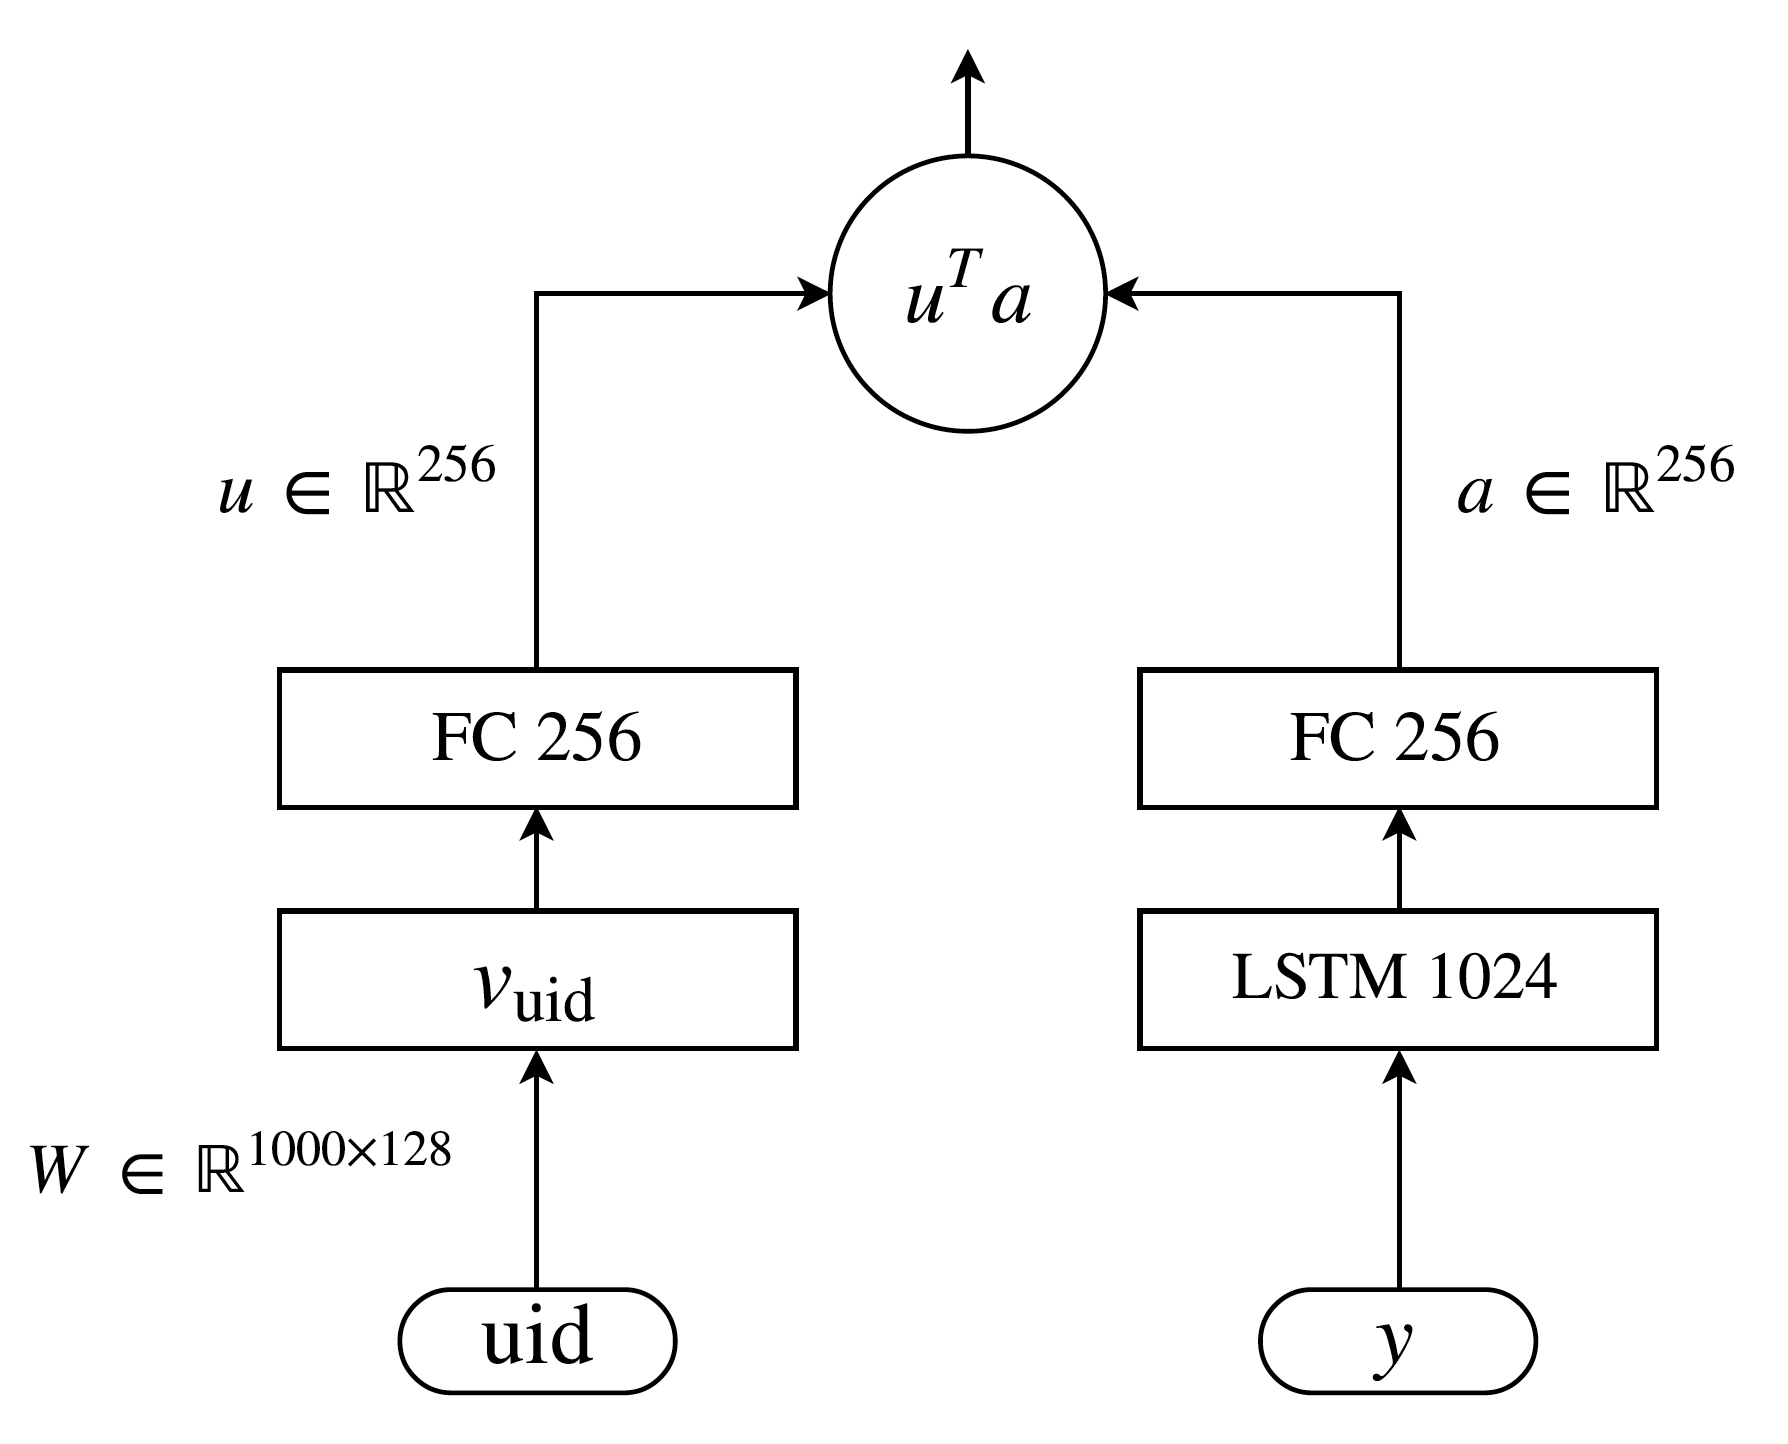
\includegraphics[scale=0.4]{imgs/dssm-belikex.png}
	\label{fig:belikex-dssm}
	\centering
\end{figure}

Заметим, что модель похожести обучается один раз и фиксируется. Обозначим диалоговую модель, обученную на $\mathcal{D}_g$ за $G_g$. Для широты эксперимента модель $G_g$ была дообучена на выборке $\mathcal{D}_s$ классическим способом (см. \eqref{crossentropy}). Обозначим её за $G_s$.

В дальнейшем зафиксируем идентификатор пользователя в модели $D_\psi(\text{uid}, y)$ равным идентификатору тех. поддержки, а также её веса $\psi$ и будем писать $D(y)$.


\subsection{Решение}

В данном эксперименте методом обучения с подкреплением был выбран Self-critical Sequence Training (SCST), где в качестве награды выступает $D(\hat{y})$.

Модель $G_g$ была дообучена в трёх различных вариациях на различных выборках:

\begin{enumerate}
	\item \textbf{SCST-ON-SUPPORT}. На выборке $\mathcal{D}_s$ модель дообучена по аналогии с $G_s$, но по функционалу потерь \eqref{eq:rl-belikex-loss}. Значение $\alpha = 1.0$.
	\item \textbf{SCST-ON-USERS}. Аналогично предыдущему пункту, но на выборке $\mathcal{D}_u$.
	\item \textbf{SCST-ON-HIGH-REWARDED}. Из выборки $\mathcal{D}_u$ были отобраны только те пары $(x, y)$, для которых выполнялось условие $D(y) > 0.5$. Объём результирующей выборки составил 22000 примеров. Значение $\alpha = 2.0$.
\end{enumerate}

Три выборки в этих вариациях содержат разное количество ''хороших'' реплик, то есть реплик, похожих на пользователя тех. поддержки. В $\mathcal{D}_s$ количество высоконаграждаемых реплик минимально, в $\mathcal{D}_u$ максимально. Третий вариант промежуточный.

\subsection{Результаты}

В Табл. \ref{table:belikex-dssm-similar} находятся примеры фраз $y$ с наибольшими значениями $D(y) = 1.0$ от пользователей, отличных от выбранного в эксперименте. Видно, что модель хорошо выучила отображение в семантическое пространство и пригодна для использования в качестве функции награды.

\begingroup
\renewcommand{\arraystretch}{1.5}
\begin{center}
	\begin{table}[htbp]
		\caption{Фразы из выборки $ \mathcal{D}_u $ с максимальной похожестью 1.0.}
		\label{table:belikex-dssm-similar}
		\begin{tabulary}{\textwidth}{|L|}
			\hline
			Фраза\\
			\hline \hline
			Ответили в ДМ. \\
			\hline
			Приносим извинения за возможные неудобства. \\
			\hline
			сейчас все решим, приносим извинения за неудобства. \\
			\hline 
			позвольте еще раз принести Вам наши извинения за доставленные неудобства.\\
			\hline
			Спасибо, что помогли нам провести работу над ошибками. \\
			\hline
			Если Вы оставляли заявку на тестирование, появится после праздников.  \\
			\hline
			Ответили вам в ЛС. \\
			\hline
			Оператор видит ситуацию происходящую с номером и сможет вам помочь. \\
			\hline
			наши специалисты делают все возможное, чтобы решить данный вопрос в кратчайшие сроки. \\
			\hline
			Также мы акцентировали внимание специалистов на важности оперативного обслуживания покупателей. \\
			\hline
			Можно Ваши ФИО и дату рождения нам в ЛС? Разберемся \\
			\hline
			Вы также находитесь в Плесецком районе? Если да, то приносим извинения за временные неудобства :\text{(} \\
			\hline
			город Астана, верно? Вы часто там бываете? Если мы примем запрос по номеру для проверки? \\
			\hline
			вас соединят с оператором, который видит всю ситуацию с номером и вам обязательно поможет. \\
			\hline
			ожалуйста, расскажите о проблеме подробнее. Какой именно сбой и где (нас. пункт, улица, дом)? \\
			\hline
		\end{tabulary}
	\end{table}
\end{center}
\endgroup

В Табл. \ref{table:belikex-ppl} представлены значения перплексии для всех моделей на валидационных выборках, соответствующих $\mathcal{D}_g$ и $\mathcal{D}_s$. Строка BASELINE соответствует модели $G_g$, а строка LLH-FINETUNED -- модели $G_s$. В Табл. \ref{table:belikex-dssm-score} представлены значения метрики avgD.


\begingroup
\renewcommand{\arraystretch}{1.8}
\begin{table}
	\centering
	\begin{tabular}{|l|c|c|}
		\hline
		& $\mathcal{D}_g$                   &   $\mathcal{D}_s$ \\
		\hline 
		BASELINE & 6.330 & 14.269 \\ 
		\hline
		LLH-FINETUNED & 24.308 & 1.040 \\
		\hline 
		SCST-ON-SUPPORT & 17.574 & 1.175 \\
		\hline
		SCST-ON-USERS & 8.178 & 26.691 \\
		\hline
		SCST-ON-HIGH-REWARDED & 24.305 & 1.283 \\
		\hline
	\end{tabular}
	\caption{Значения перплексии для моделей из эксперимента BeLikeX.}
	\label{table:belikex-ppl}
\end{table}
\endgroup

\begingroup
\renewcommand{\arraystretch}{1.8}
\begin{table}
	\centering
	\begin{tabular}{|l|c|c|}
		\hline
		& $\mathcal{D}_g$                   &   $\mathcal{D}_s$ \\
		\hline 
		BASELINE & 0.0130 & 0.0484 \\ 
		\hline
		LLH-FINETUNED & 0.6743 & 0.9546 \\
		\hline 
		SCST-ON-SUPPORT & 0.7798 & 0.8967 \\
		\hline
		SCST-ON-USERS & 0.0192 & 0.0183 \\
		\hline
		SCST-ON-HIGH-REWARDED & 0.3357 & 0.9331 \\
		\hline
	\end{tabular}
	\caption{Значения avgD для моделей из эксперимента BeLikeX.}
	\label{table:belikex-dssm-score}
\end{table}
\endgroup


Модель, дообученная методом SCST на всей выборке $\mathcal{D}_u$, даёт неудовлетворительные результаты, сравнимые с бейзлайном. Связать это можно с минимальным процентом реплик в $\mathcal{D}_u$ с высокой наградой. Модель, дообученная на $\mathcal{D}_s$ выигрывает у бейзлайна LLH-FINETUNED на выборке $\mathcal{D}_g$ за счёт эффективного исследования при обучении стратегии.

Интересным результатом с промежуточными значениями метрик является модель, дообученная на выборке ответов с высокими наградами. При специфическом контексте из области тех. поддержки модель уверенно отвечает в нужном стиле. Однако и на общей выборке она пытается генерировать фразы, похожие на ответы тех. поддержки.

Для качественного анализа в Табл. \ref{table:belikex-model-answers} приведены ответы моделей SCST-ON-SUPPORT и SCST-ON-HIGH-REWARDED на различные контексты. Первая модель переобучилась по выборку $\mathcal{D}_s$ и на общие контексты генерирует неуместные ответы в стиле тех. поддержки. Вторая же не потеряла ''знание'' об общих репликах и генерирует уместные ответы на общие контексты, при этом отвечая в нужном стиле на контексты области тех. поддержки.

\begingroup
\renewcommand{\arraystretch}{1.8}
\begin{center}
	\begin{table}[htbp]
		\caption{Ответы различных моделей в эксперименте BeLikeX.}
		\label{table:belikex-model-answers}
		\begin{tabulary}{\textwidth}{|L|L|L|}
			\hline
			Контекст & SCST-ON-SUPPORT & SCST-ON-HIGH-REWARDED \\
			\hline \hline
			привет! \textbf{EOS} как дела? & коллеги помогите , пожалуйста , только в личные сообщения ( город , улица , поселок , лк ) & у нас нет света , но хорошо . \\
			\hline
			интернет не работает что делать?' \textbf{EOS} & коллеги помогите , пожалуйста , более подробно какие сложности с использованием . & здравствуйте ! если возникли сложности , то вы можете проверить баланс ? \\ 
			\hline
			что такое любовь ? \textbf{EOS} & коллеги, пожалуйста , базовые всей компании & все ахахахаххахаха \\
			\hline 
			здравствуйте ! с какими сложностями столкнулись ? \textbf{EOS} уже все хорошо , спасибо & если возникнут вопросы , пожалуйста , обращайтесь & если будут вопросы , пишите ! \\
			\hline
			какой у вас регион ? \textbf{EOS} томская область & какой у вас регион ? & проверьте , пожалуйста \\
			\hline
			какой у вас регион ? \textbf{EOS} как дела ? & проверьте , пожалуйста & :d все хорошо , но ограничения к сведению \\
			\hline
			ты любишь учиться ? \textbf{EOS} я обожаю ! а ты ? & какой у вас регион ? & нет , но к сожалению , не могу сказать одно время , да . \\
			\hline
		\end{tabulary}
	\end{table}
\end{center}
\endgroup


\pagebreak
\section{Заключение}

\subsection{Итоги работы}
В данной работе предложен новый подход для дообучения нейросетевых диалоговых моделей с помощью методов обучения с подкреплением. На двух задачах: запрета обсценной лексики в ответе и требования отвечать ''в стиле'' технической поддержки продемонстрирована эффективность метода в сравнении с классическими бейзлайнами. Подведём итоги по проделанной работе:

\begin{enumerate}
	\item Была обучена рекуррентная диалоговая модель на выборке субтитров к англоязычным фильмам. Такое базовое решение генерировало 136 обсценных слов в среднем на 1000 предложений. 
	\item Затем, модель была дообучена с помощью A2C метода обучения с подкреплением, продемонстрировав снижение обсценной лексики в 6 раз, до 21 слова в среднем на 1000 предложений. При этом потеря в перплексии составила всего 4\%, что является незначительной потерей. Таким образом, A2C метод позволил эффективно дообучить диалоговую модель под поставленную задачу за счёт исследования в процессе генерации слов.
	\item Была обучена диалоговая модель на выборке русскоязычных диалогов из социальной сети Twitter.
	\item Была обучена модель ''похожести'' фразы на пользователя. Качественно показано, что она хорошо отбирает реплики, похожие по смыслу и лексике на фразы технической поддержки.
	\item Диалоговая модель была дообучена по методу SCST, в качестве награды была взята модель ''похожести''. Продемонстрирована эффективность дообучения, нужный результат был достигнут.
\end{enumerate}

\subsection{Дальнейшие исследования}

Дальнейшие исследования можно разделить в соответствиии с двумя проведёнными экспериментами:

\begin{enumerate}
	\item \textbf{BePolite}. На практике, собранный список обсценных слов может не покрыть всё их множество. Поэтому интересно проанализировать, насколько модель воспринимает семантику того, что ей запрещают говорить. Например,  можно взять кластер синонимичных обсценных слов, часть из которых оставить в списке, а вторую часть убрать. После дообучения можно посмотреть, насколько реже стали использоваться те слова, которые убрали из списка.
	\item \textbf{BeLikeX}. В проведенном исследовании модель похожести на вход принимала только индентификатор пользователя и реплику, но никак не учитывала контекст в диалоге. Возможно, обуславливание модели на контекст поможет при дообучении.
	
	Также, интересно использовать наработки из соперничающих генеративных сетей, а именно, трактовать модель похожести как дискриминатор, а диалоговую модель как генератор, и дообучать обоих по соперничающему функционалу потерь.
\end{enumerate}

\newpage
\bibliography{library}
%\bibliographystyle{abbrv}
\bibliographystyle{unsrt}


\end{document}
